% Ustawienia dokumentu
\documentclass[11pt,oneside]{book}
\usepackage[T1]{fontenc}
\usepackage[utf8]{inputenc}
\usepackage{graphicx}
\usepackage{amsmath,amssymb,amsfonts}
\usepackage{txfonts}
\usepackage{listings}
\usepackage[polish]{babel}
\usepackage{fullpage}
\usepackage{color}
\usepackage{caption}
\usepackage[pdftex]{hyperref}
\usepackage{pdfpages}

\hypersetup{
  colorlinks,
  urlcolor=blue,
  citecolor=red,
  linkcolor=red
}
\urlstyle{rm}
\linespread{1.2}  % interlinia
\captionsetup[figure]{name=Rys.}
\renewcommand\lstlistlistingname{Spis Listingów}

% definicje typów
\definecolor{LightGray}{cmyk}{0,0,0,0.1}
\newtheorem{definition}{Definicja}

% informacje o dokumencie
\author{Paweł~Placzyński}
\title{System aukcyjny w~Ruby~on~Rails}
\date{\today}

% DOKUMENT
\begin{document}


\includepdf{obrazki/strona_tytulowa.png}

\tableofcontents

\section{Cele i~problematyka pracy}

\subsection{Cele}

\subsubsection{Przybliżenie metodologii Scrum}

Jednym z~podstawowych celów pracy inżynierskiej jest przedstawienie (prezentacja) wykorzystanych w~niej technologii, narzędzi, metod itp. Ze~względu na~użycie podczas pisania mojej pracy metodologii Scrum \cite{scrumalliance} (używanej powszechnie w~małych i~średnich firmach -- nie tylko programistycznych) zamierzam opisać tę~metodologię i~zaprezentować w~prosty sposób jej przebieg.

\subsubsection{Przybliżenie (popularyzacja) technologii Ruby~on~Rails} \label{cele.ror}

Ruby~on~Rails (często nazywany RoR lub po~prostu Rails) to~framework open source do~szybkiego tworzenia aplikacji webowych stworzony głównie przez duńskiego programistę Davida Heinemeiera Hanssona w~ramach pracy nad oprogramowaniem Basecamp\footnote{Patrz: \url{http://basecamphq.com/}}. Rails to~w~pełni wyposażone środowisko do~tworzenia aplikacji internetowych opartych o~bazy danych zgodnie ze~wzorcem MVC (Model-View-Controller). Ruby~on~Rails daje programiście środowisko w~pełni oparte o~język programowania Ruby -- od~Ajax'a dostępnego w~widokach (View), do~zapytania i~odpowiedzi w~kontrolerach i~logice biznesowej modeli.


Tuż po~pojawieniu się Ruby~on~Rails na~forum publicznym okrzyknięto go~sensacyjnym. Tim O'Reilly, Założyciel O'Reilly Media mówił\footnote{Źródło: \url{http://www.rubyonrails.pl/cytaty}} ,,Ruby on Rails jest przełomem w~dziedzinie programowania aplikacji internetowych. Potężne aplikacje, których tworzenie do~tej pory zabierało tygodnie czy miesiące, są~teraz tworzone dosłownie w~kilka dni.''


Niestety -- w~ciągu ostatnich trzech lat spadło zainteresowanie technologią Ruby~on~Rails (patrz wykres \ref{fig.wykres.googleresearch}). Programiści coraz rzadziej sięgają po~ten produkt wybierając nowsze rozwiązania takie jak Django\footnote{Patrz: \url{http://www.djangoproject.com/}} napisane w~języku Python\footnote{Patrz: \url{www.python.org}}. Nadzieją na~poprawienie tej sytuacji jest nowo wydana -- trzecia wersja frameworku Ruby~on~Rails oraz~ciągły rozwój dodatków -- wtyczek \texttt{gem}. Dlatego też chcę przybliżyć tę~technologię i~zachęcić do~jej używania.

\begin{figure}[!t]
\centering
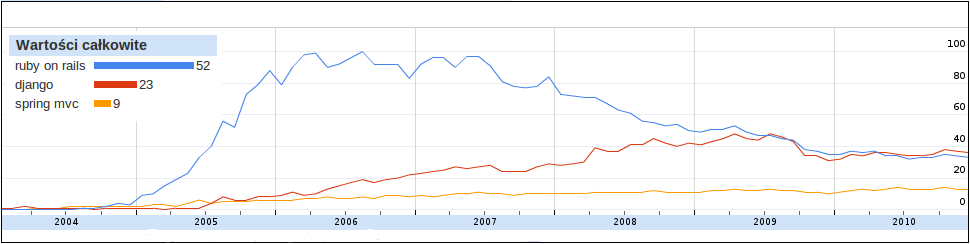
\includegraphics[width=\textwidth]{obrazki/googleresearch.png}
\caption{Statystyka wyszukiwarki Google na~temat znanych aplikacji szkieletowych (źródło: \url{http://www.google.com/insights/search/\#cat=5\&q=Ruby\%20on\%20Rails\%2CDjango\%2CSpring\%20MVC\&cmpt=q}).}
\label{fig.wykres.googleresearch}
\end{figure}

Liczby na~wykresie \ref{fig.wykres.googleresearch} wskazują, ile wyszukiwań przeprowadzono na~podstawie określonego hasła w~porównaniu do~łącznej liczby wyszukiwań przeprowadzonych w~Google w~tym czasie. Wartości te~nie odzwierciedlają bezwzględnej liczby wyszukiwań, ponieważ dane są~znormalizowane i~przedstawione na~skali od~0 do~100. Każdy punkt na~wykresie jest dzielony przez wartość najwyższego punktu. Jeśli ilość danych jest za~mała, podawana jest wartość 0. Liczby wyświetlane nad wykresem obok wyszukiwanych haseł stanowią podsumowania lub wartości łączne\footnote{Źródło: \url{http://www.google.com/support/insights//bin/answer.py?hl=pl\&answer=87285}}.

\subsubsection{Opis zastosowania technologii Ruby~on~Rails w~problemie stworzenia systemu aukcyjnego}

Technologia Ruby~on~Rails umożliwia proste tworzenie aplikacji webowych dowolnego typu. Dla zaprezentowania jej możliwości wybrałem system aukcyjny jako przykład aplikacji webowej stworzonej w~tym środowisku. Wybór ten nie jest przypadkowy -- do~tej pory nie znalazłem przykładowego systemu aukcyjnego napisanego przy użyciu aplikacji szkieletowej Ruby~on~Rails\footnote{Jedynym możliwym gotowym rozwiązaniem dla wykorzystania aplikacji webowej w~celu wystawiania aukcji/prowadzenia licytacji jest zastosowanie wtyczki % TODO nazwa i url
dla systemu CMS % TODO nazwa i url CMS - chyba spree
napisanego w~Ruby~on~Rails.}.


Pomysł jednak nie jest nowatorski -- w~sieci oraz~w~wielu pozycjach książkowych znajdują się przykłady wykonania sklepów internetowych, które są~w~budowie bardzo podobne do~systemów aukcyjnych.


System aukcyjny to~niezwykle rozwlekły i~obszerny temat. Projekt tego typu zatem może być bardzo rozbudowany. Właśnie z~tego względu zakładam, że~mój projekt nie będzie ,,dokończony''. Celem nie jest tu~wykonanie całego projektu ,,od~początku do~końca'' a~jedynie prezentacja możliwości jakie oferuje Ruby~on~Rails.

\subsubsection{Przedstawienie prototypu systemu aukcyjnego}

Wraz ze~stworzeniem prototypu systemu aukcyjnego prezentuję podstawowe rozwią\-zania dla tego rodzaju problemu. Zagadnienie stworzenia systemu aukcyjnego jest problemem typowym dla dziedziny inżynierii oprogramowania. Wymaga wybrania i~opracowania rozwiązań technicznych i~technologicznych oraz~określenia metodyki pracy nad danym zagadnieniem.


Stworzony przeze mnie prototyp jest swego rodzaju prezentacją zastosowanych w~nim technologii oraz~przykładowych rozwiązań.

\subsubsection{Ocena możliwości wdrożenia proponowanych rozwiązań}

Do~pełnego przedstawienia cyklu pracy nad projektem wykonanym w~technologii Ruby~on~Rails potrzebne jest przedstawienie metod wdrożenia aplikacji webowej oraz~zaproponowanie sposobu jej konserwacji. W~tym celu mam zamiar przybliżyć jedne z~najprostszych znanych mi sposobów wdrożenia aplikacji Ruby~on~Rails.


\chapter{Technologie i~narzędzia}

\textit{W~poniższym rozdziale opisane są~technologie oraz~narzędzia, które wykorzystane zostały podczas realizacji systemu aukcyjnego w~Ruby~on~Rails.}

\section{Technologie zastosowane w~pracy}

W~itym podrodziale wymienione zostały technologie zastosowane podczas tworzenia serwisu aukcyjnego będącego celem pracy.

\subsection{Ruby oraz Ruby~on~Rails} \label{technologie.baza}

\subsubsection{Ruby 1.9.3} \label{technologie.ruby}

\textit{Ruby} (ang.~rubin) to interpretowany, w~pełni obiektowy i~dynamicznie typowany język programowania stworzony w~1995 roku przez Yukihiro Matsumoto (pseudonim Matz). Wersja 1.9.3 cechuje się szybszym interpreterem, mniejszą konsumpcją zasobów oraz~drobnymi poprawkami w~standardowych bibliotekach języka.

\subsubsection{Ruby~on~Rails 3.1.0} \label{technologie.ror}

\textit{Ruby~on~Rails}\cite{ror} (często nazywany \textit{RoR} lub po~prostu \textit{Rails}) to~framework \textit{open~source} służący do~szybkiego tworzenia aplikacji webowych stworzony głównie przez duńskiego programistę Davida Heinemeiera Hanssona w~ramach pracy nad oprogramowaniem \textit{Basecamp}\cite{basecamp}. \textit{Rails} to~w~pełni wyposażone środowisko do~tworzenia aplikacji internetowych opartych o~bazy danych zgodnie ze~wzorcem \textit{MVC} (ang.~Model-View-Controller). \textit{Ruby~on~Rails} daje programiście środowisko w~pełni oparte o~język programowania \textit{Ruby} -- od~\textit{Ajax} dostępnego w~widokach (ang.~View), do~zapytania i~odpowiedzi w~kontrolerach i~logice biznesowej modeli.


Tuż po~pojawieniu się \textit{Ruby~on~Rails} na~forum publicznym okrzyknięto go~sensacyjnym. Tim O'Reilly, Założyciel O'Reilly Media mówił\cite{cytaty} ,,Ruby on Rails jest przełomem w~dziedzinie programowania aplikacji internetowych. Potężne aplikacje, których tworzenie do~tej pory zabierało tygodnie czy miesiące, są~teraz tworzone dosłownie w~kilka dni.''


Niestety -- w~ciągu ostatnich trzech lat spadło zainteresowanie technologią \textit{Ruby~on~Rails} (rys.~\ref{fig.wykres.googleresearch}). Programiści coraz rzadziej sięgają po~ten produkt wybierając nowsze rozwiązania takie jak \textit{Django}\cite{django} napisane w~języku \textit{Python}\cite{python}. Nadzieją na~poprawienie tej sytuacji jest nowo wydana -- trzecia wersja frameworku \textit{Ruby~on~Rails} oraz~ciągły rozwój dodatków -- wtyczek \texttt{gem}.

\begin{figure}[!t]
\centering
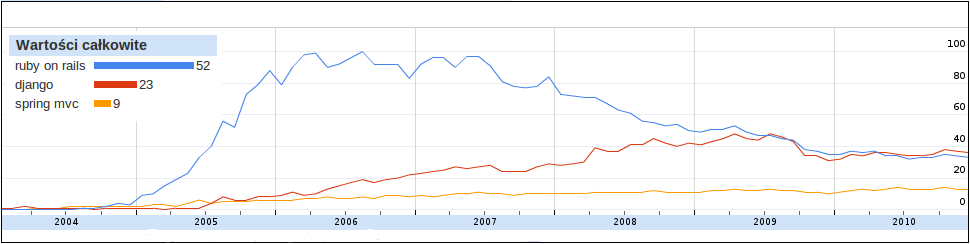
\includegraphics[width=\textwidth]{obrazki/googleresearch.png}
\caption[Statystyki Google na temat aplikacji szkieletowych]{Statystyka wyszukiwarki Google na~temat znanych aplikacji szkieletowych\cite{google.stats}}
\label{fig.wykres.googleresearch}
\end{figure}

\subsubsection{RSpec + Cucumber}

\textit{RSpec}\cite{rspec} to~narzędzie do~testownia oprogramowania pod względem testów jednostkowych oraz~behawioralnych przydatne w~realizowaniu projektów \textit{Test Driven Developement} oraz~\textit{Behavior Driven Developement}. Narzędzie \textit{Cucumber}\cite{cucumber} pozwala na~testowanie oprogramowania na podstawie tzw. scenariuszy -- dokumentów napisanych w języku naturalnym opisujących krok po~kroku funkcjonalności projektu.

% gemy, rozszerzenia, pluginy, dodatki, etc.

\subsection{Gemy i pluginy} \label{technologie.gemy}

\texttt{Gem} to~wtyczka (ang.~plugin), rozszerzenie dla aplikacji napisanych w jezyku \textit{Ruby}. \textit{Gemy} są~w~łatwy sposób zarządzane przez narzędzie \texttt{rubygems} pozwalające na pobieranie dowolnej wersji \textit{gemów} z~repozytoriów.


Do~realizacji celów pracy wykorzystano następujące wtyczki:

\begin{enumerate}
  \item \texttt{haml}\cite{haml} to plugin pozwalajacy na~użycie eleganckiego metajęzyka opisującego strukturę dokumentów HTML.
  \item \texttt{sass}\cite{sass} to podobny w działaniu do \texttt{haml} plugin obsługujący szablony CSS.
  \item \texttt{device}\cite{devise} to system obsługi autentyfikacji użytkowników (rejestracja, sesje, zarządzanie hasłami itp.) dla frameworku Ruby~on~Rails.
  \item \texttt{will\_paginate}\cite{will.paginate} to plugin obsługujący paginację stron.
  \item \texttt{tiny\_mce}\cite{tiny.mce} to plugin napisany w~języku JavaScript pozwalający na~użycie wewnętrznego edytora HTML na~stronach internerowych.
  \item \texttt{sqlite3}\cite{sqlite3} to relacyja baza danych z~możliwością użycia jezyka zapytań SQL; jest lekka i~szybka, czechuje się tym że bazy danych przechowywane są~w~osobnych plikach. Posiada swój własny adapter na~platformę Ryby~on~Rails.
\end{enumerate}

% technologie webowe

\subsection{Technologie W3 i poboczne} \label{technologie.web}

\textit{W3}\cite{w3} to~organizacja mająca na~celu opracowanie i~publikację dokumentacji standardów rządzących technologiami wykorzystywanymi do~tworzenia stron internetowych.

\begin{enumerate}
  \item \texttt{XHTML5}\cite{html5doc} (ang.~HyperText Markup Language version 5) jest językiem określającym strukturę stron internetowych. Składniowo bazuje on~na~języku XML (jest podzbiorem języka XML). Wersja piąta zapewnia kompatybilność wsteczną względem poprzednich wersji, a~przy tym precyzuje niejasności wersji 4 powodujące nieoczekiwane zachowanie wyświetlanych obiektów w~niektorych przeglądarkach.
  \item \texttt{CSS3}\cite{css3doc} (ang.~Cascade Style Sheet version 3). CSS3 jest językiem określającym wygląd elementów języka XML jaki wyświetlany jest w~przeglądarce. Wersja 3 zapewnia kilka dodatkowych opcji, jak np. \textit{grid layouts} (szablony pozycjonowane na bazie siatki)\footnote{\url{http://www.w3.org/TR/css3-grid/}}, \textit{shadows and rounded borders} (cienie obiektów, zaokrąglenia obramowania)\footnote{\url{http://www.w3.org/TR/css3-background/}}, itp.
  \item \texttt{JavaScript} jest lekkim, zorientowanym obiektowo wieloplatformowym językiem skryptowym. JavaScript, mimo że~nie jest użyteczny jako samodzielny język, został stworzony z~myślą o~łatwym zagnieżdżaniu w~innych produktach i~aplikacjach, jak na~przykład przeglądarki internetowe. JavaScript może zostać powiązany z~wewnętrzną strukturą danego środowiska dając programiście swobodną kontrolę nad jego elementami.
  \item \texttt{AJAX} (ang. Asynchronous JavaScript and XML) to technologia tworzenia aplikacji internetowych, w~której interakcja użytkownika z~serwerem odbywa się bez przeładowywania całego dokumentu, w~sposób asynchroniczny. Ma~to~umożliwiać bardziej dynamiczną interakcję z~użytkownikiem niż w~tradycyjnym modelu, w~którym każde żądanie nowych danych wiąże się z~przesłaniem całej strony HTML.
  \item \texttt{jQuery}\cite{jquery} (z.~ang. query -- zapytanie) -- lekka biblioteka programistyczna dla języka JavaScript, ułatwiająca korzystanie z~JavaScript (w~tym manipulację drzewem DOM). Kosztem niewielkiego spadku wydajności w~stosunku do~profesjonalnie napisanego kodu w~niewspomaganym JavaScripcie pozwala osiągnąć interesujące efekty animacji, dodać dynamiczne zmiany strony, wykonać zapytania AJAX. Większość pluginów i~skryptów opartych o~jQuery działa na~stronach nie wymagając zmian w~kodzie HTML (np.~zamienia klasyczne galerie złożone z~miniatur linkujących do~obrazków w~dynamiczną galerię). Wszystkie efekty osiągnięte z~pomocą jQuery można osiągnąć również bez jej użycia. Jednak kod okazuje się nieporównywalnie dłuższy i~bardziej skomplikowany.
\end{enumerate}


\section{Narzędzia użyte podczas pisania pracy} \label{narzedzia}

Realizujac założenia pracy inżynierskiej użyto podczas jej tworzenia całej gamy narzędzi. Proces tworzenia przebiegał na~systemie operacyjnym GNU~Linux\footnote{\url{http://www.kerner.org}} (dystrybucja Ubuntu\cite{ubuntu}).

\subsection{Kontrola pracy w~Scrum}

Narzędzia użyte do kontroli przebiegu pracy nad projektem:

\subsubsection{Git}

\textit{Git}\cite{git} to~rozproszony system kontroli wersji. Stworzył go~Linus Torvalds jako narzędzie wspomagające rozwój jądra Linux. Git stanowi wolne oprogramowanie i~został opublikowany na~licencji GNU~GPL w~wersji~2.


Pierwsza wersja narzędzia Git została wydana 7~kwietnia~2005 roku, by~zastąpić poprzednio używany w~rozwoju Linuksa, niebędący wolnym oprogramowaniem, system kontroli wersji \textit{BitKeeper}.


Wiele projektów używa \textit{Git} jako system kontroli wersji, zarówno nowo powstające, jak i~migrują do~niego z~innego systemu kontroli wersji (na~przykład~CVS lub SVN). Do~największych i~najbardziej znanych projektów o~otwartym źródle, należy wymienić: jądro Linuksa oraz~podprojekty z~nim związane, a~także GNU~Hurd, GNOME, GTK+, GStreamer, KDE, GIMP, Perl, Qt, Ruby~on~Rails, Samba, Wine, Xfce, Xorg, jQuery, YUI, Erlang. Również część serwisów internetowych używa \textit{Git} do~rozwijania swojego kodu (a~część z~niego jest publicznie dostępna), m.in.~Reddit (otwarte źródła), digg, facebook.


Kilka systemów operacyjnych korzysta z~Gita do~zarządzania całą dystrybucją oraz~dodatkowymi programami w~nie wchodzącymi: Arch Linux, Android, Fedora, Maemo, MeeGo, OLPC~XO-1, openSUSE oraz DragonFly~BSD. Dystrybucje Debian oraz~Ubuntu używają Gita do~rozwijania programów oraz~zmian w~programach zewnętrznych dla wielu (choć nie wszystkich) pakietów.

\subsubsection{tig}

\texttt{tig} to~narzędzie \texttt{ncurses} służące do~prostego zarządzania repozytorium \texttt{git}. Jest dobrą alternatywą dla wbudowanego w~pakiet narzędzi systemu Git \texttt{gitg}, pozwalającą na~wykorzystanie identycznych funkcjonalności w konsoli.

\subsubsection{ticgit}

\texttt{ticgit}\cite{ticgit} to~prosty issue tracker (narzędzie do zarządzania zadaniami zwiazanymi z~projektem) działajacy jako rozszerzenie dla systemu kontroli wersji Git; zapisuje zmiany w~trackingu w oddzielnej gałęzi repozytorium Git projektu. Pozwala to~na~przechowywanie dokumentacji dotyczącej rozwoju projektu wraz z~kodami źródłowymi.

\texttt{ticgit} jest aplikacją konsolową, aczkolwiek istnieje rozszerzenie pozwalając na~zarządzanie zadaniami \texttt{ticgit} przy pomocy przeglądarki internetowej i~prostego interfejsu webowego\cite{ticgitweb}.

\subsection{Środowisko programistyczne}

Oprócz systemu operacyjnego potrzebne są także narzędzia do zarządzania środowiskiem programistycznym (język programowania, bibilioteki, wtyczki, itp.), a także narzędzia wspomagające programowanie jak edytory tekstu, konsole, itp.).

\subsubsection{zsh + GNU~Screen}

Większość pracy nad projektem napisanym przy pomocy frameworku Ruby~on~Rails odbywa się w~konsoli. Jako powłoki użyto powłoki Open-Source \texttt{zsh}\cite{zsh}. Powłoka ta~udostępnia rozbudowany i~przyjazny użytkownikowi system podpowiedzi (system ten zintegrowany jest z~wieloma poleceniami konsoli, w~tym z~narzędziami systemu kontroli wersji Git), jak również udogodnienia dotyczące historii wykonywanych poleceń, autokorektę oraz~szereg opcji konfiguracji zachowania i~wyglądu.


\texttt{screen}\cite{screen} jest narzędziem pozwalającym na~sprawne zarządzanie uruchomionumi powłokami/poleceniami. Pozwala na:

\begin{itemize}
  \item przełączanie się pomiędzy uruchomionymi powłokami/poleceniami,
  \item pracę w~kilku oknach (widokach),
  \item odłączanie się (deteach) i~pozwalanie na kontynuację wykonywanych poleceń (opcja przydatna podczas pracy zdalnej),
  \item kopiowanie/wklejanie/przeszukiwanie ekranu konsoli,
  \item wyświetlanie informacji o~systmie/procesach w~dolnej linijce ekranu,
\end{itemize}

\subsubsection{Vim}

\textit{Vim}\cite{vim} według oficjalnej interpretacji oznacza \texttt{vi improved}. Jest to~wieloplatformowy klon edytora tekstu \texttt{vi}, napisany przez Brama Moolenaara, holenderskiego programistę.


Vim jest edytorem dającym się w~dużym stopniu konfigurować. W~efekcie Vim może być surowy i~nieprzyjazny jak jego protoplasta lub przeciwnie: cieszyć intelekt i~oko bogactwem funkcji lub kolorów. Istnieje także możliwość rozbudowania umiejętności tego edytora poprzez dodawanie wtyczek (napisanych własnoręcznie lub pobranych ze~strony domowej projektu).


Vim w ostatnich latach był kilkukrotnie wybierany na~najpopularniejszy edytor tekstowy wśród czytelników Linux Journal, wyprzedzając m.in.~Emacsa.

\subsubsection{RVM}

\textit{RVM}\cite{rvm} to~system kontrolii wersji języka Ruby. Pozwala na~zainstalowanie wielu implementacji i~wersji tego języka na~lokalnej maszynie oraz~proste zarządzanie wtyczkami Gem dla tych implementacji. Umożliwia proste przełączanie się pomiędzy wersjami języka.

\subsubsection{IRB}

\textit{IRB} to~interaktywna konsola języka Ruby udostępniana wraz z~tym językiem. Jest ona podobna w~działaniu do~konsoli języka Python, a~zatem udostępnia szereg opcji pozwalających na~testowanie małych porcji kodu jezyka Ruby w~,,biegu''. Możliwe jest także skonfigurowanie zachowań konsoli IRB przy pomocy skryptów napisancych w~języku Ruby (na~przykład~kolorowanie składni, formatowanie wyjścia konsoli).

\subsubsection{Sqliteman}

Sqliteman\cite{sqliteman} to~narzędzie do~zarządzania bazami danych Sqlite3. Oferuje graficzny interfejs, pozwalający na~szybkie przeglądanie/edycję zawartości bazy danych.

\subsection{Wdrożenie}

Do~pełnego przedstawienia cyklu pracy nad projektem wykonanym w~technologii Ruby~on~Rails potrzebne jest przedstawienie metod wdrożenia aplikacji webowej oraz~zaproponowanie sposobu jej konserwacji. W~tym celu przybliżono jedno z~najprostszych sposobów wdrożenia aplikacji Ruby~on~Rails.

\subsubsection{Heroku}

\textit{Heroku}\cite{heroku} to~serwis pozwalający na~uruchamianie i~konserwację projektów napisanych w~języku Ruby ,,w~chmurze''.


\textit{Heroku} wykorzystuje \textit{cloud-computing} do~wdrażania alpikacji webowych, opartych na~interfejsie \textit{Ruby~Rack} (aplikacji Ruby~on~Rails, Sinatra, itp.). Pozwala to~na~odrzucenie zbędnego planowania oraz~konfiguracji/konserwacji środowisk uruchomieniowych. Zmniejsza to~koszt zatrudnienia administratorów, a~także koszt sprzętu lub niezbędnych usług (połączenie internetowe, certyfikaty, domeny)


\textit{Heroku} nie jest jedyną taką usługą dostępną dla programistów Ruby, jednakże tylko ono~pozwala na~założenie niewielkich aplikacji testowych.


\chapter{Metodyka pracy}

\textit{W~tym rozdziale opisana została organizacja pracy nad projektem, konwencje użyte podczas tworzenia aplikacji oraz~standardy pracy w~zespole programistycznym.}

\section{Metodyka Scrum} \label{scrum}

Zastosowaną przeze mnie metodyką pracy jest Scrum \cite{scrumalliance} (z~ang. scrum -- przepychanka, młyn). Jest to~jedna z~wielu pochodnych metodyki programowania zwinnego \cite{agile1} (z~ang. agile programming).

\subsection{Programowanie zwinne} \label{scrum.agile}

Programowanie zwinne jest popularną metodą pracy w~wielu firmach parających się programowaniem. Dla wyjaśnienia czym tak naprawdę jest wystarczy nam odczytać definicję z~Wikipedii \cite{agile2}:

\begin{quote}
Programowanie zwinne (z~ang. Agile software development) -- grupa metodyk wytwarzania oprogramowania opartego o~programowanie iteracyjne (model przyrostowy). Wymagania oraz~rozwiązania ewolu\-ują przy współpracy samozarządzalnych zespołów, których celem jest przeprowadzanie procesów wytwarzania oprogramowania. Pojęcie zwinnego programowania zostało zaproponowane w 2001 w~Agile Manifesto\footnote{Patrz: \url{agilemanifesto.org/principles.html}}.


Generalnie metodyka oparta jest o~zdyscyplinowane zarządzanie projektem, które zakłada częste inspekcje wymagań i rozwiązań wraz z~procesami adaptacji (zarówno specyfikacji jak i~oprogramowania). Metodyka ta~najczęściej znajduje zastosowanie w~małych zespołach programistycznych, w~których nie występuje problem komunikacji, przez co~nie trzeba tworzyć rozbudowanej dokumentacji kodu. Kolejne etapy wytwarzania oprogramowania zamknięte są~w~iteracjach, w~których za~każdym razem przeprowadza się testowanie wytworzonego kodu, zebranie wymagań, planowanie rozwiązań itd. Metoda nastawiona jest na~szybkie wytwarzanie oprogramowania wysokiej jakości.


Metoda nastawiona jest na~bezpośrednią komunikację pomiędzy członkami zespołu, minimalizując potrzebę tworzenia dokumentacji. Jeśli członkowie zespołu są~w~różnych lokalizacjach, to~planuje się codzienne kontakty za~pośrednictwem dostępnych kanałów komunikacji (wideokonferencja, e-mail itp.).
\end{quote}

Więcej informacji można znaleźć na~stronie \url{www.agileprogramming.org} \cite{agile1}.

\subsection{Scrum} \label{scrum.scrum}

Omówię tu~po~krótce metodykę Scrum wykorzystaną podczas realizacji założeń części praktycznej pracy. Metodyka Scrum opiera się na~ścisłych iteracjach, w~których realizowane są~założenia projektowe. Każda iteracja zaczyna się tzw. Sprint~Meeting'iem (z~ang. Sprint meeting -- ,,spotkanie w~biegu'')\footnote{Więcej na~temat metodyki Scrum można znaleźć na~stronie \url{www.scrumalliance.org}}.

\begin{figure}[!t]
\centering
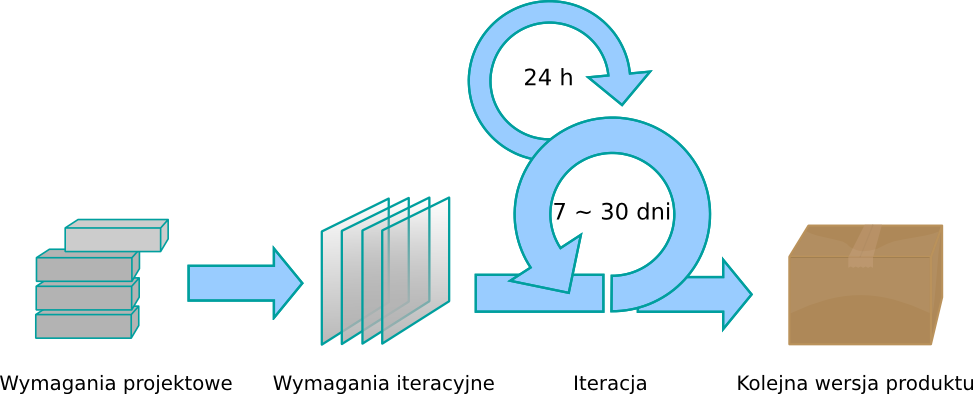
\includegraphics[width=\textwidth]{obrazki/scrum.png}
\caption{Schemat pracy w~kolejnych iteracjach metodyki Scrum (opracowane na~podstawie: \url{http://effectiveagiledev.com/Portals/0/800px-Scrum\_process\_svg.png}).}
\label{fig.rysunek.scrum}
\end{figure}

\subsubsection{Definicje pojęć dla metodyki Scrum} \label{scrum.definicje}

\begin{definition}[Deweloper]
Deweloperem (z~ang. developer -- konstruktor, inwestor) nazywamy osobę bądź firmę\footnote{tu: osobę}, która zaangażowana jest w~realizację czynności związanych z~procesem wytwarzania oprogramowania. Zwykle deweloperem nazywamy członka zespołu projektowego -- programistę.
\end{definition}

\begin{definition}[Iteracja]
Iteracją nazywamy cykl w~procesie wytwarzania oprogramowania, który zamknięty zostaje poprzez zrealizowanie pewnego celu.
\end{definition}

\begin{definition}[Ticket]
Zadania przydzielone zespołowi projektowemu określamy mianem ticketu. Ticket (z~ang. ticket -- bilet) określa jakie obowiązki zostały narzucone na~poszczególnych deweloperów. Jest zwykle odzwierciedleniem żądań i~zaleceń od~klienta.
\end{definition}

\subsubsection{Role} \label{scrum.role}

Główne role jakie można wymienić w~zespole Scrum to:

\begin{enumerate}
  \item Zespół programistyczny (z~ang. The Team) -- wykonawcy projektu, deweloperzy w~liczbie do~9 osób. Do ich obowiązków należy ocena trudności zadań -- ticketów -- realizujących założenia projektowe, realizacja tych zadań oraz~zgłaszanie błędów, trudności itp.~zaistniałych w~projekcie.
  \item Właściciel projektu (z~ang. Product Owner) -- jest to~osoba, firma, grupa itp.~będąca zleceniodawcą (klientem) zatrudniającym zespół programistyczny do~zrealizowania projektu. Zasadniczą rolą właściciela projektu jest przedstawianie założeń, wymagań co~do~projektu, rewizja wykonanych zadań tegoż zespołu oraz~konsultowanie zmian. Gdy właścicielem projektu jest jakaś większa jednostka (firma, spółka, grupa itp.) wtedy wyznaczany jest reprezentant odpowiedzialny za~wyżej wymienione czynności.
  \item Mistrz młyna (z~ang. Scrum Master) -- osoba odpowiedzialna za~komunikację pomiędzy zespołem programistycznym a~właścicielem projektu. Do~jej obowiązków należy przede wszystkim: ustalanie sprint meeting'ów, zgłaszanie intencji zespołu programistycznego, wysyłanie powiadomień o~zmianach w~założeniach itp.
\end{enumerate}

\subsubsection{Rozpoczęcie pracy w~Scrum} \label{scrum.poczatki}

Zanim zostanie otworzona pierwsza iteracja -- sprint -- należy dokładnie przemyśleć i~omówić możliwości grupy projektowej oraz~skonfrontować je~z~wymaganiami klienta. W~tym celu organizowane jest spotkanie inicjujące pracę nad projektem. Na~takim spotkaniu powinny zostać omówione następujące kwestie:

\begin{enumerate}
  \item Omówienie metody pracy z~klientem -- klient powinien wiedzieć jak pracuje zespół  czego może się po~nim spodziewać.
  \item Prezentacja założeń projektowych -- tu~zespół programistyczny dowiaduje się jakie są~postawione wobec niego oczekiwania.
  \item Rewizja założeń projektowych -- zespół programistyczny ma~tu~szansę wypowiedzieć się na~temat kolejnych założeń -- związanych z~nimi trudności, konfrontacja z~umiejętnościami (czego trzeba się ,,douczyć'' a~co~jest zagwarantowane poprzez doświadczenie zespołu).
  \item Wycena projektu oraz~ustalenie licencji jego użytkowania.
\end{enumerate}

Po~omówieniu tych zagadnień klient może zdecydować, czy taki sposób pracy mu~odpowiada. W tym momencie jest w~stanie oszacować jak długo będzie współpracował nad projektem z~tą~grupą projektową, a~co~za~tym idzie -- jaką ilość pieniędzy może przeznaczyć w~poszczególnych etapach tworzenia projektu.

\subsubsection{Sprint meeting} \label{scrum.sprintmeeting}

Sprint meeting zamyka jedną iterację i~rozpoczyna następną. Podczas sprint meeting'u realizowane są zatem: sprawdzenie poprawności wykonanych zadań z~poprzedniej iteracji oraz przedyskutowanie planu pracy w następnej iteracji. Pozwala to klientowi na~pełną kontrolę nad procesem wytwarzania projektu. Do~najważniejszych kwestii omawianych na~sprint meeting'u należą:

\begin{enumerate}
  \item Sprawdzenie stanu wykonanych zadań -- jeśli zadania zostały dostarczone klientowi jako wykonane, to~klient może je~zweryfikować pod względem ich poprawności. Każde takie zadanie może zostać zaakceptowane (wtedy oznaczone zostaje jako wykonane) bądź nie (Zadanie odrzucone wymaga poprawki -- klient może zdecydować, co~powinno być w~tej sytuacji wykonane. Jeżeli klient ma~wystarczająco funduszy na~wykonanie poprawek wtedy może zlecić poprawkę, jeśli nie, to~zadanie może zostać ,,zamrożone'' i~czekać na~pieniądze potrzebne do~jego realizacji. Oczywiście klient może także zaniechać realizacji zadania.).
  \item Określenie wymagań projektowych -- klient wymienia swoje oczekiwania względem projektu. Wymagania te~zostają skonfrontowane z~możliwościami zespołu programistycznego (,,tego nie da~się zrobić'', ,,to~jest za~trudne'', ,,to~wymaga lepszego sprzętu'', ,,realizacja tego zadania zajmie \ldots'', ,,koszta tego zadania wyniosą około \ldots'', albo: ,,to~jest proste'', ,,znamy się na~tym'' itp.). Zwykle zaistniałe trudności w~realizacji zadań kończą się kompromisem. Po~określeniu możliwości realizacji wymagań tworzone są~zadania.
  \item Określenie zadań dla grupy projektowej -- po~,,wycenie'' możliwości deweloperów względem wymagań tworzone są~zadania. Zwykle rozbija się je~na~prostsze, wymagające mniej czasu (według zasady ,,dziel i~zdobywaj'') -- uzyskuje się wtedy płynność w~realizacji zadań, a~praca nad konkretnym wymaganiem podzielona jest pomiędzy członkami zespołu.
  \item Przydzielenie zadań -- klient po~określeniu i~sprecyzowaniu zadań określa ich priorytet. Niektóre zadania są~ważniejsze -- te~oznaczane są~jako zadania przypisane nadchodzącej iteracji -- nad tymi zadaniami grupa projektowa będzie w~najbliższym czasie pracować. Zadania te~zostają następnie wybierane przez konkretnych deweloperów jako te, które będą przez nich realizowane. Jeżeli po~zakończonej iteracji zostaną zadania nie wykonane przez nikogo oznacza to, że~grupa nie nadąża z~tempem pracy narzuconym przez klienta.
  \item Ustalenie ,,dostępności'' deweloperów w~najbliższej iteracji. Członkowie zespołu mogą z~różnych powodów nie móc pracować w~pewnym okresie czasu. Z~tego względu pod koniec sprint meeting'u należy ustalić ile godzin pracy każdy deweloper może przeznaczyć na~najbliższą iterację. Pozwala to~określić ,,siłę'' zespołu oraz~długość iteracji. W~szczególnych przypadkach iteracje mogą zostać przeniesione bądź zawieszone ,,do~odwołania''.
\end{enumerate}

\subsection{Narzędzia Scrum} \label{scrum.narzedzia}

Narzędzi, które wspomagają pracę w~metodyce Scrum jest wiele. Przykładem mogą być tzw. Issue Tracker'y -- środowiska do~zarządzania ticketami. Dobrym przykładem takiego Issue Trackera jest PivotalTracker\footnote{\url{www.pivotaltracker.com}}. Pozwala on~na~kontrolowanie zadaniami poprzez oznaczanie ich jako wykonanych, bieżących itp. Przykładowe zastosowanie tego narzędzia w~pracy nad projektem przedstawia rysunek \ref{fig.rysunek.pivotal}.

\begin{figure}[!t]
\centering
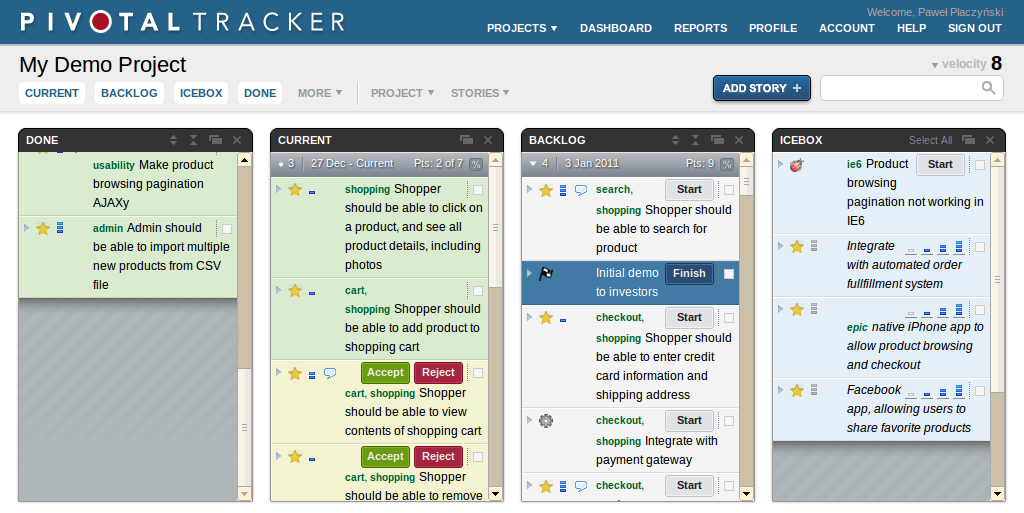
\includegraphics[width=\textwidth]{obrazki/pivotal.png}
\caption{Zastosowanie narzędzia PivotalTracker w~pracy nad projektem (źródło: \url{www.pivotaltracker.com}).}
\label{fig.rysunek.pivotal}
\end{figure}

Innym przykładem narzędzia wspomagającego pracę w~projekcie Scrum są~testy jednostkowe i~funkcjonalne aplikacji (patrz rozdział \ref{dokumentacja.testy}). Służą one tutaj przede wszystkim rewizji zaimplementowanej funkcjonalności a zatem sprawdzeniu poprawności wykonania zadania. Testy takie są~zatem udokumentowaniem wykonanej pracy przez dewelopera.


\section{Dokumentacja projektu} \label{dokumentacja}

Projekty systemów informatycznych mają to~do~siebie, że~rozwijają się niezwykle szybko. Rozwój projektu związany jest niestety z~powiększaniem objętości projektu -- zarówno merytorycznej, jak i~czysto fizycznej (ilość linijek kodu, ilość plików). Problem pojawia się, gdy projekt jest zbyt ,,duży'', żeby programista mógł rozumieć wszystko to, co~się w~nim dzieje. Rozwiązaniem dla tego problemu jest tworzenie dokumentacji.


W~projektach typu \textit{OpenSource} dokumentacja jest niezwykle ważnym czynnikiem usprawniającym pracę programistów w~nich pracujących. Dobrze napisana dokumentacja sprawia, że~nowe osoby zaczynające pracę w~projekcie mogą łatwiej i~szybciej zapoznać się ze~strukturą, działaniem oraz~organizacją projektu. Jest to~szczególnie przydatne, gdy istnieje potrzeba edycji jedynie niewielkiego fragmentu projektu. Co~więcej -- osoby zajmujące się już od~dłuższego czasu pracą w~takim projekcie nie muszą pamiętać wszelkich zagadnień z~nim związanych.


\subsection{Kod aplikacji} \label{dokumentacja.kod}

Najlepszą dokumentacją dla systemu informatycznego jest kod aplikacji. To~właśnie on~realizuje wszystkie założenia projektowe, algorytmy lub cykle pracy projektu. Prawidłowo napisany kod może powiedzieć więcej niż nie jedna dokumentacja -- tu~dowiadujemy się, jak naprawdę działa interesujący nas moduł i~mamy pewność, że~nie padniemy ofiarą nieporozumień. Pod pojęciem ,,prawidłowo napisany kod'' rozumie się spełnienie następujących założeń:

\begin{itemize}
  \item ,,trzymanie się'' konwencji określającej osnowę dokumentu, zawierającego kod,
  \item stosowanie zrozumiałych nazw dla wszelkich struktur (nazwy klas, metod, zmiennych),
  \item tworzenie krótkich i~treściwych fragmentów kodu oraz~rozbijanie większych partii kodu na~mniejsze.
\end{itemize}

Wszystkie te kroki mają na celu sprawienie, że~kod stanie się bardziej czytelny. Poniżej omówiono te~trzy kroki nieco dokładniej w~zastosowaniu dla języka Ruby.

\subsubsection{Konwencja} \label{dokumentacja.konwencja}

Język Ruby ze~względu na~swoją składnię jest niezwykle czytelny, a~co~za~tym idzie, kod w~nim napisany jest łatwy w~zrozumieniu. Składnia Rubiego przypomina pseudokod (listing \ref{code.pseudocode}).

  \lstset{language=Ruby, caption=Przykład prostej składni języka Ruby -- algorytm DFS, basicstyle=\ttfamily\footnotesize, numbers=left, numberstyle=\footnotesize, captionpos=b, backgroundcolor=\color{LightGray}}
  \begin{lstlisting}[label={code.pseudocode}]
  def dfs node, value, queue
    return false if node.nil?
    return true if node.data == value
    queue.push node.right_neighbor unless node.right_neighbor.nil?
    queue.push node.left_neighbor unless node.left_neighbor.nil?
    dfs queue.pop, value, queue
  end
  \end{lstlisting}

Niestety sama składnia nie jest najważniejsza w~dokumentowaniu projektów. Powyższy przykład można przecież przepisać w~inny sposób (listing \ref{code.unclear}

  \lstset{language=Ruby, caption=Algorytm DFS z~zastosowaniem braku konwencji formatu, basicstyle=\ttfamily\footnotesize, numbers=left, numberstyle=\footnotesize, captionpos=b, backgroundcolor=\color{LightGray}}
  \begin{lstlisting}[label={code.unclear}]
  def dfs node, value, queue
  return false if node.nil?; if node.data == value
  return true
  end; queue.push node.right_neighbor unless \\
    node.right_neighbor.nil?
  unless node.left_neighbor.nil?
  queue.push node.left_neighbor; end
  dfs queue.pop, value, queue
  end
  \end{lstlisting}

Przykład ten jest mniej czytelny, a~co~za~tym idzie, trudniej jest dowiedzieć się, za~co~dany fragment kodu jest odpowiedzialny. W~celu uzyskania ,,przejrzystości'' kodu stosuje się konwencje zapisu -- ogólnie przyjęte zasady mówiące o~tym, jak powinien wyglądać kod i~jak ten kod formatować. Język Ruby posiada swoją konwencję o~nazwie \textit{The Ruby Style} \cite{therubyway}, która określona jest następująco:

\begin{enumerate}
  \item Formatowanie:
  \begin{enumerate}
    \item Używaj zawsze kodowania ASCII lub UTF8.
    \item Używaj dwóch spacji jako wcięć (nigdy tabulatur).
    \item Staraj się kończyć wiersz w~stylu używanym w~systemach Unix (LF -- 0x0A).
    \item Używaj spacji przed i~po~operatorach, po~przecinkach, po~dwukropkach, po~średnikach, przed i~po~\{ oraz~po~\}.
    \item Nie używaj spacji po~( oraz~[. Nie używaj spacji przed~] oraz~).
    \item Używaj dwóch spacji przed modyfikatorem warunku (\texttt{if}/\texttt{unless}/\texttt{while}/\texttt{until}/\texttt{resque}).
    \item Wcięcie dla słowa kluczowego \texttt{when} powinno być tak głębokie, jak dla \texttt{case}.
    \item Użyj pustego wiersza przed zwracaną wartością w~metodzie (chyba, że~ma~ona tylko jeden wiersz), a~także przed słowem kluczowym \texttt{def}
    \item Używaj \textit{RDoc} do~dokumentacji API. Nie wstawiaj pustego wiersza pomiędzy komentarz a~komentowany blok.
    \item Użyj pustego wiersza do~podzielenia dużych metod na~logiczne fragmenty.
    \item Staraj się, aby~każdy wiersz miał mniej niż 80 znaków.
    \item Unikaj białych znaków na~końcu wiersza.
  \end{enumerate}
  \item Składnia:
  \begin{enumerate}
    \item Użyj \texttt{def} z~ nawiasami, gdy są~podane argumenty.
    \item Nie używaj \texttt{for}, chyba, że~robisz to~celowo.
    \item Nie używaj \texttt{then}.
    \item Użyj ,,\texttt{when x;} \ldots'' dla jednolinijkowego wyrażenia \texttt{case}.
    \item Użyj \texttt{\&\&}/\texttt{||} dla wyrażeń boolowskich, \texttt{and}/\texttt{or} do~kontroli przepływu.
    \item Unikaj wielolinikowej instrukcji \texttt{?:}, użyj \texttt{if}.
    \item Zaniechaj użycia nawiasów przy wywołaniu metod, ale użyj ich podczas wywołania ,,funkcji'' (na~przykład~gdy używasz zwracanej wartości w~tym samym wierszu).
    \item Używaj raczej \mbox{\texttt{\{} \ldots \texttt{\}}} niż \mbox{\texttt{do} \ldots \texttt{end}}. Wielolinijkowe bloki \mbox{\texttt{\{} \ldots \texttt{\}}} są~poprawne: używając \texttt{\}} na końcu bloku wiemy, że~kończy się blok a~nie instrukcja \texttt{if}/\texttt{while}/\ldots. Używaj \mbox{\texttt{do} \ldots \texttt{end}} do~kontroli przepływu (na~przykład~zadania \texttt{rake}, bloki \texttt{sinatra}).
    \item Unikaj używania słowa kluczowego \texttt{return}, jeśli nie jest potrzebne.
    \item Unikaj kontynuacji linii (\texttt{$ \backslash $}), jeśli nie musisz.
    \item Używanie zwracanej wartości przez operator \texttt{=} jest na miejscu.
    \item Używaj operatora \texttt{||=}.
    \item Używaj wyrażeń regularnych typu ,,non-OO''.  Nie bój się używać \texttt{=~}, \texttt{\$0-9}, \texttt{\$~}, \texttt{\$`} oraz~\texttt{\$'} jeśli potrzebujesz.
  \end{enumerate}
  \item Nazewnictwo:
  \begin{enumerate}
    \item Używaj \textit{snake\_case} jako stylu nazywania metod.
    \item Używaj \textit{CamelCase} jako stylu nazywania klas i~modułów (pozostaw akronimy takie jak HTTP, RFC, XML z~wielkich liter).
    \item Używaj SCREAMING\_SNAKE\_CASE jako stylu nazywania stałych.
    \item Długość nazwy zwykle określa kontekst wykorzystania. Używaj jednoliterowych zmiennych jako parametrów bloków/metod według schematu:\\
      \texttt{a}, \texttt{b}, \texttt{c}, \texttt{o}: dowolny obiekt;\\
      \texttt{d}: katalog;\\
      \texttt{e}: element (klasy \texttt{Emumerable} oraz~pochodnych);\\
      \texttt{ex}: wyjątek;\\
      \texttt{f}: plik:\\
      \texttt{i}, \texttt{j}: indeksy;\\
      \texttt{k}: klucz tablicy asocjacyjnej;\\
      \texttt{m}: metoda;\\
      \texttt{r}: zwracana wartość krótkich metod;\\
      \texttt{s}: tekst;\\
      \texttt{v}: wartość elementu tablicy asocjacyjnej;\\
      \texttt{x}, \texttt{y}, \texttt{z}: liczby;\\
      Ponadto, pierwsza litera klasy obiektu może posłużyć za~nazwę takiej zmiennej.

    \item Używaj nazw zaczynających się od~\texttt{\_} dla nieużywanych zmiennych.
    \item Używając \texttt{inject} dla krótkich bloków nazywaj argumenty \texttt{|a, e|} (akumulator, element).
    \item Definiując operatory dwuargumentowe, nazywaj argument jako ,,other''.
    \item Używaj raczej \texttt{map} niż \texttt{collect}, \texttt{find} niż \texttt{detect}, \texttt{find\_all} niż \texttt{select} oraz~\texttt{size} niż \texttt{length}.
  \end{enumerate}
  \item Komentarze:
  \begin{enumerate}
    \item Komentarze dłuższe niż słowo rozpoczynają się z~wielkiej litery i~używane są zasady interpunkcji.
    \item Używaj dwóch spacji po każdej kropce w komentarzu.
    \item Unikaj niepotrzebnych komentarzy.
  \end{enumerate}
  \item Pozostałe:
  \begin{enumerate}
    \item Pisz kod przyjazny dla opcji \texttt{ruby -w}.
    \item Unikaj tablic asocjacyjnych jako opcjonalnych parametrów.
    \item Unikaj długich metod.
    \item Unikaj długich list parametrów.
    \item Używaj konstrukcji \texttt{def self.}\textit{metoda} dla zdefiniowania metod singletonów.
    \item Staraj się rozwijać funkcjonalność standardowych metod.
    \item Unikaj \texttt{alias} -- używaj \texttt{alias\_method}.
    \item Używaj \texttt{OptionParser} do~parsowania skomplikowanych opcji wejścia konsoli a~\texttt{ruby -s} dla rozwiązań trywialnych.
    \item Staraj się zachować zgodność wielu wersji interpretera.
    \item Unikaj zbędnego metaprogramowania.
  \end{enumerate}
  \item Ogólne zasady:
  \begin{enumerate}
    \item Programuj w~sposób funkcjonalny.
    \item Nie wydziwiaj z~używaniem argumentów metod -- chyba, że~wiesz co robisz.
    \item Nie zmieniaj funkcjonalności standardowych bibliotek pisząc własne.
    \item Nie programuj zachowawczo \cite{zachowawcze}.
    \item Postaraj się zachować prostotę kodu.
    \item Nie nadużywaj projektowania.
    \item Ale także nie pozostaw swojej pracy niezaprojektowanej.
    \item Unikaj błędów.
    \item Poczytaj o innych konwencjach, aby móc rozwinąć tę.
    \item Bądź konsekwentny.
    \item Używaj prostych rozwiązań.
  \end{enumerate}
\end{enumerate}

Stosowanie tej konwencji zapewni, że~napisany kod będzie zgodny z~ogólnym standardem.

\subsubsection{Nazewnictwo w~kodzie} \label{dokumentacja.nazewnictwo}

Aby zrozumieć istotę działania projektu należy zrozumieć mechanizmy i~algorytmy rządzące jego logiką. Zakładając, że~chcemy utworzyć dobrą dokumentację projektu, trzeba tak napisać kod, by~był zrozumiały -- jak pseudokod opisujący algorytm. W~tym celu wystarczy, że~wszelkie obiekty w~ kodzie, nazwiemy tak, by~ich użycie w~kontekscie było zrozumiałe a~ich rola jasna. W~trakcie pisania kodu najtrudniejszą kwestią jest nazywanie obiektów, a~nie -- jak to~się powszechnie uznaje -- rozwiązanie logiki systemu.

\subsection{Komentarze} \label{dokumentacja.komentarze}

Komentarze w~kodzie to~dobrzy sposób na~wyjaśnienie zasadności użycia algorytmów, bądź struktury API poszczególnych elementów kodu. Stosowanie komentarzy pozwala także wyróżnić, ważniejsze dla ,,czytelnika'' elementy kodu.

\subsubsection{RDoc} \label{dokumentacja.rdoc}

Istnieje wiele konwencji dotyczących~formy komentarzy. Format komentarzy ma~znaczenie nie tylko podczas czytania kodu -- może on~posłużyć pośrednio do~wygenerowania pełnej dokumentacji API przy użyciu odpowiednich narzędzi.


Komentarze w~języku Ruby mogą być dwojakiego formatu (listing \ref{code.comments}).

  \lstset{language=Ruby, caption=Komentarze w~języku Ruby, basicstyle=\ttfamily\footnotesize, numbers=left, numberstyle=\footnotesize, captionpos=b, backgroundcolor=\color{LightGray}}
  \begin{lstlisting}[label={code.comments}]
    # Komentarz jednolinijkowy rozpoczyna sie
    # od znaku krzyzyka.

    =begin
      Blok komentarza.
      Taki blok rozpoczyna sie od znacznika "=begin"
      a konczy na znaczniku "=end".
      Komentarze jednolinijkowe sa jednak czesciej
      uzywane.
    =end
  \end{lstlisting}


Narzędzie \textit{RDoc} \cite{rdoc} to~narzędzie konsolowe generujące dokumentację API w~zadanym formacie (standardowo jest to~HTML) na~podstawie kodu oraz~komentarzy w~nim zawartych. Aby wygenerować taką dokumentację wystarczy wpisać w~konsoli:

\mbox{\texttt{\$ rdoc <opcje> [plik...] }}

\textit{RDoc} wygeneruje czytelną dokumentację nawet bez komentarzy w~kodzie.

\subsection{Testy} \label{dokumentacja.testy}

Testy to~dodatkowe aplikacje sprawdzające poprawność logiki projektu. Zasadniczą ich funkcją jest dowiedzenie, że~dana funkcjonalność została zaimplementowana poprawnie.


Testować w~aplikacji można wszystko, jednak dobrze jest ustalić, co~chce się uzyskać poprzez napisanie testów. Biorąc pod uwagę powyższe kryterium testy dzieli się na:

\begin{enumerate}
 \item \textit{Testy jednostkowe} -- sprawdzają poprawność modułów ,,silnika'' aplikacji. Za~pomocą testów jednostkowych testuje się zwykle klasy, metody, stany maszyny, poprawność algorytmów, wejścia i~wyjścia strumieni.
 \item \textit{Testy behawioralne} -- odpowiadają na~pytanie: ,,co~się stanie, gdy zrobimy \ldots''. Testują zachowanie aplikacji -- reakcję na~żądania, efekty działania zdarzeń (takich jak, na przykład, wypełnienie formularza).
\end{enumerate}

\subsubsection{Testy jednostkowe RSpec} \label{dokumentacja.rspec}

\textit{RSpec} \cite{rspec} jest narzędziem do~tworzenia testów jednostkowych dla aplikacji napisanych w~języku Ruby. Jego składnia jest prosta, a~testy w~nim napisane -- czytelne (listing \ref{code.simple_test}).

  \lstset{language=Ruby, caption=Test \textit{RSpec} testujący klasę \texttt{Array}, basicstyle=\ttfamily\footnotesize, numbers=left, numberstyle=\footnotesize, captionpos=b, backgroundcolor=\color{LightGray}}
  \begin{lstlisting}[label={code.simple_test}]
  describe Array do
    describe "#push" do
      it "puts a value at the end of array" do
        array = Array.new
        value = "Some value"
        array.push value
        array.last.should == value
      end
    end
  end
  \end{lstlisting}

W~pierwszej kolejności podaje się opis testu -- krótką informację o~tym, co~testujemy i~jakie są oczekiwania względem testowanego obiektu. Wewnątrz bloku testu realizuje się przypadek użycia obiektu. W~każdym momencie można sprawdzić, czy interesujący nas stan obiektu jest zgodny z~naszymi oczekiwaniami. W~tym celu używa się metod \texttt{should} oraz~\texttt{should\_not}.


Testy uruchamiamy podając w~konsoli polecenie \texttt{rspec} oraz~plik z~napisanymi testami:

\mbox{\texttt{\$ rspec nazwa\_pliku\_testu.rb}}

Trzeba pamiętać, że~testy powinny mieć dostęp do~logiki projektu -- na~przykład~poprzez użycie instrukcji \texttt{require}. Efektem działania testu z~przykładu \ref{code.simple_test} widoczny jest na listingu \ref{code.simple_test_results}

\lstset{language=bash, caption=Efekt uruchomienia testu jednostkowego z~przykładu \ref{code.simple_test}, basicstyle=\ttfamily\footnotesize, numbers=left, numberstyle=\footnotesize, captionpos=b, backgroundcolor=\color{LightGray}}
\begin{lstlisting}[label={code.simple_test_results}]
.

Finished in 0.00258 seconds
1 example, 0 failures
\end{lstlisting}

Aby zrozumieć, co~stało się podczas testowania, można zmienić format wyjścia na~bardziej przyjazny (listing \ref{code.test_pretty}).

\lstset{language=bash, caption=Efekt uruchomienia testu jednostkowego z~opcją \texttt{----format d}, basicstyle=\ttfamily\footnotesize, numbers=left, numberstyle=\footnotesize, captionpos=b, backgroundcolor=\color{LightGray}}
\begin{lstlisting}[label={code.test_pretty}]
Array
  #push
    puts a value at the end of array

Finished in 0.0029 seconds
1 example, 0 failures
\end{lstlisting}

Jak widać \texttt{rspec} poinformował o~tym, które testy ,,przeszły'' -- czyli, które z~testowanych funkcjonalności spełniły oczekiwania.

\subsubsection{RSpec jako dokumentacja}

Przykład \ref{code.simple_test} mówi dość dużo o~sposobie użycia elementów logiki projektu. Testy jednostkowe są~tak naprawdę przypadkami użycia tychże elementów. Co~więcej -- przypadki te~realizują się zgodnie z~założeniami twórcy takiego projektu (uruchomione testy ,,przechodzą''). Oznacza to, że~są one dobrą dokumentacją działania i~sposobu użycia poszczególnych obiektów logiki projektu.

\subsubsection{Dokumentacja poprzez testy behawioralne} \label{dokumentacja.cucumber}

Skoro testy jednostkowe są~swego rodzaju dokumentacją, to~także testy behawioralne mogą nią być. Oczywiście ze~względu na~inny cel testy behawioralne będą dokumentować projekt z~innej perspektywy. Testy te~określają zachowanie aplikacji, a~zatem kwestię ściśle związane z~użytkowaniem. W~praktyce testy behawioralne są~stosowane dla określenia wymagań ze~strony klienta -- zleceniodawcy projektu.


Istnieje kilka narzędzi, przy pomocy których można napisać i~przeprowadzić testy behawioralne. Można do~tego użyć \texttt{rspec} oraz~\texttt{Test::Unit} (czyli narzędzi wykorzystywanych przy pisaniu testów jednostkowych). Dla dobrej czytelności oraz~eleganckiego formatu użyto narzędzia \textit{Cucumber} \cite{cucumber}.


\textit{Opisane powyżej metody pracy z~projektem zostały zastosowane w~systemie aukcyjnym, będącym celem pracy.\\\\W~następnym rozdziale zaprezentowany zostanie proces tworzenia systemu aukcyjnego oraz~opisany zostanie utworzony prototyp.}

\chapter{Projekt systemu aukcyjnego}

\textit{W~rozdziale tym opisany został proces tworzenia aplikacji \texttt{auctioneer}, a~także końcowy efekt i~wnioski dotyczące stworzonego systemu aukcyjnego.}

\section{Wprowadzenie}

\subsubsection{Opis zastosowania technologii Ruby~on~Rails w~problemie stworzenia systemu aukcyjnego}

Technologia Ruby~on~Rails umożliwia proste tworzenie aplikacji webowych dowolnego typu. Dla zaprezentowania jej możliwości wybrałem system aukcyjny jako przykład aplikacji webowej stworzonej w~tym środowisku. Wybór ten nie jest przypadkowy -- do~tej pory nie znalazłem przykładowego systemu aukcyjnego napisanego przy użyciu aplikacji szkieletowej Ruby~on~Rails\footnote{Jedynym możliwym gotowym rozwiązaniem dla wykorzystania aplikacji webowej w~celu wystawiania aukcji/prowadzenia licytacji jest zastosowanie wtyczki % TODO nazwa i url
dla systemu CMS % TODO nazwa i url CMS - chyba spree
napisanego w~Ruby~on~Rails.}.


Pomysł jednak nie jest nowatorski -- w~sieci oraz~w~wielu pozycjach książkowych znajdują się przykłady wykonania sklepów internetowych, które są~w~budowie bardzo podobne do~systemów aukcyjnych.


System aukcyjny to~niezwykle rozwlekły i~obszerny temat. Projekt tego typu zatem może być bardzo rozbudowany. Właśnie z~tego względu zakładam, że~mój projekt nie będzie ,,dokończony''. Celem nie jest tu~wykonanie całego projektu ,,od~początku do~końca'' a~jedynie prezentacja możliwości jakie oferuje Ruby~on~Rails.

\subsubsection{Przedstawienie prototypu systemu aukcyjnego}

Wraz ze~stworzeniem prototypu systemu aukcyjnego prezentuję podstawowe rozwią\-zania dla tego rodzaju problemu. Zagadnienie stworzenia systemu aukcyjnego jest problemem typowym dla dziedziny inżynierii oprogramowania. Wymaga wybrania i~opracowania rozwiązań technicznych i~technologicznych oraz~określenia metodyki pracy nad danym zagadnieniem.


Stworzony przeze mnie prototyp jest swego rodzaju prezentacją zastosowanych w~nim technologii oraz~przykładowych rozwiązań.


\section{Przebieg pracy}

W~tym podrozdziale opiszę fazy tworzenia projektu i~jego rozwoju.

\subsection{Przygotowanie środowiska pracy}

Pierwszym krokiem do~stworzenia systemu aukcyjnego w~technologii Ruby~on~Rails jest przygotowanie środowiska, w~którym projekt bedzie tworzony. Pominięto tutaj proces instalacji systemu operacyjnego.

\subsubsection{Instalacja narzędzi}

Większość narzędzi wymienionych w~rozdziale \ref{narzedzia} Narzędzia można zainstalować wpisując w~konsoli następujące polecenie:


\texttt{sudo apt-get install zsh screen ack-grep vim ruby git git-core tig ticgit ticgitweb sqlite3 sqlite3-dev sqliteman curl}


(Polecenie to~zadziała na~Ubuntu~11.10 oraz na~Debianie~Squeeze. Na~innych dystrybucjach zamiast \texttt{apt-get} należy użyć innego manadżera pakietów dostępnego dla danej dystrybucji. Oczywiście nazwy pakietów także mogą się różnić)

\subsubsection{Zarządzanie wersją Ruby -- RVM}

W~celu zainstalowania \textit{RVM} należy wpisać w~konsoli:


\texttt{bash -s stable < <(curl -s https://raw.github.com/wayneeseguin/rvm/master/binscripts/rvm-installer)}


Aby zainstalować Ruby w~wersji 1.9.3 należy wpisać:


\texttt{rvm install 1.9.3}


Po~konfiguracji i~kompilacji zadanej wersji Ruby należy tylko przełączyć się na~nią:


\texttt{rvm --default use 1.9.3}


Polecenie \texttt{ruby -v} powinno wypisać \texttt{ruby 1.ruby9.ruby93p0 (2011-10-30 revision 33570) [x86\_64-linux]}.

\subsubsection{Instalacja Ruby~on~Rails oraz niezbędnych wtyczek}

Ruby~on~Rails instalujemy wpisując:


\texttt{gem install rails}


W~ten sposób można już utworzyć pierwszy, podstawowy projekt Ruby~on~Rails:


\texttt{rails new auctioneer}


Polecenie to~utworzy katalog auctioneer zawierający podstawowe elementy każdego projektu Ruby~on~Rails.

\lstset{language=bash, caption=Zawartość katalogu \textit{auctioneer}, basicstyle=\ttfamily\footnotesize, captionpos=b, backgroundcolor=\color{LightGray}} \label{code.railsdir}
\begin{lstlisting}
app
app/models
app/views
app/views/layouts
app/controllers
app/helpers
app/assets
app/assets/stylesheets
app/assets/javascripts
app/assets/images
app/mailers
script
vendor
vendor/plugins
vendor/assets
vendor/assets/stylesheets
db
config
config/environments
config/locales
config/initializers
log
public
doc
test
test/integration
test/fixtures
test/functional
test/unit
test/performance
tmp
tmp/cache
tmp/cache/assets
lib
lib/tasks
lib/assets
\end{lstlisting}

Aby zainstalować konieczne do~dalszego działania wtyczki należy wyedytować plik \texttt{Gemfile} dopisując linijki z~nazwami oraz numerami wersji wtyczek.

\lstset{language=ruby, caption=Plik \texttt{Gemfile} projektu \textit{auctioneer}., basicstyle=\ttfamily\footnotesize, numbers=left, numberstyle=\footnotesize, captionpos=b, backgroundcolor=\color{LightGray}} \label{code.railsdir}
\begin{lstlisting}
source 'http://rubygems.org'

gem 'rails', '>=3.1.0'
gem 'sqlite3'

gem 'jquery-rails'
gem 'devise'
gem 'haml'
gem 'haml-rails'
gem 'formtastic'
gem 'thin'
gem 'will_paginate'
gem 'wirble', require: nil
gem 'ruby-debug19', require: nil
gem 'rspec-rails', '>= 2.6.1', group: [:development, :test]
gem 'heroku'
gem 'state_machine'

group :assets do
  gem 'sass-rails', "  ~> 3.1.0"
  gem 'coffee-rails', "~> 3.1.0"
  gem 'uglifier', '>= 1.0.3'
  gem 'therubyracer'
end

group :test do
  gem 'factory_girl_rails', '>= 1.1.0'
  gem 'cucumber-rails', '>= 1.0.2'
  gem 'capybara', '>= 1.0.1'
  gem 'database_cleaner', '>= 0.6.7'
  gem 'launchy', '>= 2.0.5'
  gem 'ruby-debug19'
  gem 'email_spec'
end
\end{lstlisting}

Po~edycji pliku \texttt{Gemfile} należy wywołać polecenie \texttt{bundle install}. Wszystkie zależności związane z~wymaganymi wtyczkami zostaną zainstalowane, a~każda zmiana w~pliku \texttt{Gemfile} wymaga ponownego uruchomienia komendy \texttt{bundle install}.

\subsubsection{Kontrola wersji Git}

W~katalogu projektu stworzonego w~poprzednim punkcie należy zainicjować system kontroli wersji wpisując polecenie:


\texttt{git init}


W~katalogu powstanie podkatalog \texttt{.git} zawierający wszystkie niezbędne informacje o historii tworzonego projektu.


W~projekcie mogą znajdować się pliki, dla~których nie chcemy przechowywać historii. Mogą to~być na~przykład pliki tymczasowe, logi, pliki backup, itp. Aby uniknąć dodawania ich do~historii rozwoju projektu należy utworzyć plik \texttt{.gitignore} i~dopisać tam niechciane pliki.


Aby zapisać bieżący stan projektu w~historii należy zaznaczyć zmiany przy pomocy polecenia \texttt{git add .} oraz wykonać commit przy pomocy \texttt{git commit}. Otworzy się domyślny edytor tekstu, w którym należy podać komentarz dotyczący zmian.

\lstset{language=bash, caption=Plik \texttt{.gitignore} projektu \textit{auctioneer}., basicstyle=\ttfamily\footnotesize, captionpos=b, backgroundcolor=\color{LightGray}} \label{code.railsdir}
\begin{lstlisting}
.sass-cache/
vendor/ruby
*~
*.swp
*.swo
tags
log/*
tmp/*
lib/mysql.rb
config/*.yml
[a-zA-Z0-9\.-_]*~
misc
capybara*
coverage
config/*.sphinx.conf
config/environments/dev_local.rb
db/sphinx/*
public/system/*
public/sitemaps/*
backup
nbproject/*
features_report.html
public/services/
public/stylesheets/all.css
public/javascripts/all.js
rerun.txt
mkmf.log
.bundle/
nohup.out
*.sqlite3
.rvmrc
doc/praca_inzynierska.pdf
\end{lstlisting}

\subsubsection{Dalsza konfiguracja}

W~poprzednich krokach została przedstawiona instalacja środowiska programistycznego dla projektu napisanego w~technologii Ruby~on~Rails. Środowisko takie jest już wystarczające i można zacząć właściwą pracę nad projektem, jednakże każde z~wyżej wymienionych narzędzi można skonfigurować według własnego uznania edytując pliki konfiguracyjne.


Do~tworzenia projektu \textit{auctioneer} użyto konfiguracji dostępnej w~repozytorium GitHub: \url{https://github.com/placek/dotfiles}.


Aby zatwierdzić taką instalację należy wykonać następujące polecenie:


\texttt{git clone git://github.com/placek/dotfiles.git; cp dotfiles/* \$HOME}

\subsection{Założenia projektu}

Zanim programista przystępuje do~pracy należy wyznaczyć szczegółowo zadania i~założenia. Wszystkie cele powinny być jasno przedstawione i~przemyślane.

\subsubsection{Założenia dotyczące projektu}

System aukcyjny powinien spełniać pewne podstawowe funkcjonalności, a~zatem powinien zapewnić możliwość:

\begin{itemize}
  \item rejestracji oraz dostępu do~konta osobom chcącym wystawiać aukcje,
  \item wystawienia aukcji oraz podania ceny minimalnej,
  \item przeglądania aukcji wraz z~ważnymi dla potencjalnych kupujących informacjami,
  \item wyszukiwania aukcji według opisu oraz podawania wyników wyszukiwania w~kolejności jaką sobie użytkownik wybierze,
  \item podbicia aukcji oraz wygrania jej na~ogólnie przyjętych zasadach.
\end{itemize}

System powinien zadbać także o~bezpieczeństwo danych użytkowników systemu oraz udostępnić możliwość administrowania danymi przez osoby uprawnione (administratorzy).

%TODO mockupy

\subsubsection{Przypadki użycia i scenariusze}

Wyróżniono następujących aktorów:

\begin{enumerate}
  \item \textit{Gość} -- odwiedzający serwis \textit{auctioneer}, nie mający na~nim osobistego konta (nie zalogowany, nie zarejestrowany). Gość może przeglądać wystawione aukcje oraz wyszukiwać z~pośród nich  interesujące go~pozycje. Gość może także zarejestrować się.
  \item \textit{Użytkownik} -- aktor posiadający osobiste konto w~serwisie \textit{auctioneer}, logujący się za~pomocą adresu email oraz hasła. Użytkownik może wykonywać akcje gościa (przeglądanie wystawionych aukcji, ich wyszukiwanie). Ponadto użytkownik posiada możliwość licytowania aukcji, wystawiana własnych aukcji i~zarządzania nimi (edycja, usuwanie, zmiana stanu aukcji).
  \item \textit{Administrator} -- aktor posiadający najwyższe uprawnienia. Może zarządzać kontami innych administratorów, jak i~kontami użytkowników (dodawanie, usuwanie kont, logowanie na~konta). Administrator ma~także pełen dostęp do~wszystkich aukcji -- może je~edytować, usuwać, zmieniać ich stan.
\end{enumerate}

Wyróżniono także następujące przypadki użycia (patrz rysunek \ref{usecase}):

\begin{enumerate}
  \item \textit{Przeglądanie wystawionych aukcji} -- podstawowa funkcjonalność systemu aukcyjnego. Każdy aktor odwiedzający serwis \textit{auctioneer} powinien mieć możliwość dostępu do~listy wystawionych aukcji oraz ich szczegółowych opisów.
  \item \textit{Wyszukiwanie aukcji pod warunkiem kryteriów wyszukiwania} -- duża ilość wystawionych aukcji może spowodować problemy ze znalezieniem interesującego odwiedzającego stronę przedmiotu aukcji. Aukcje powinny być wyszukiwane ze~względu na~nazwę i opis aukcji. Powinna być także możliwość sortowania wyników według nazwy i~ceny.
  \item \textit{Rejestracja} -- odwiedzający serwis \textit{auctioneer}, nie posiadający na~nim konta osobistego powinien mieć możliwość rejestracji. Rejestracja powinna odbywać się przy użyciu adresu email nowego użytkownika oraz hasła. Aby nowo zarejestrowane konto było aktywne (można się na~nie zalogować) należy aktywować je~poprzez wykonanie instrukcji przysłanych na~email podany podczas rejestracji.
  \item \textit{Wystawianie aukcji} -- nowo utworzona aukcja powinna zawierać tytuł (będący krótkim opisem aukcji), szczegółowy opis aukcji (detale) oraz cenę minimalną. Tak przygotowana aukcja może zostać wystawiona (upubliczniona).
  \item \textit{Licytacja} -- wystawiona aukcja zgodnie z~zamiarem wystawiającego ją~powinna posiadać cenę minimalną, od~której zaczyna się licytacja. Licytacja powinna mieć termin ważności (w~założeniu -- siedem dni od~wystawienia aukcji), po którym to wyłoniony zostaje zwycięzca aukcji -- osoba, która wylicytowała najwyższą sumę. Alternatywnym zakończeniem aukcji może być przerwanie jej przez wystawiającego przed terminem ważności.
  \item \textit{Zarządzanie aukcjami użytkownika} -- użytkownik powinien mieć możliwość edycji bądź usunięcia własnych aukcji. Powinien także mieć możliwość zmiany jej stanu (wystawienie, zamknięcie aukcji, ponowne jej wystawienie).
  \item \textit{Zarządzanie administratorami} -- aktualny administrator powinien mieć możliwość dodawania oraz usuwania innych administratorów.
  \item \textit{Zarządzanie użytkownikami} -- administrator powinien mieć możliwość edycji i~usuwania użytkowników, powinien też mieć możliwość zalogowania się jako użytkownik.
  \item \textit{Zarządzanie aukcjami} -- administrator powinien posiadać dostęp do wszystkich aukcji i~mieć możliwość ich edycji, usunięcia oraz zmiany stanu.
\end{enumerate}

\begin{figure}[hbt]
  \begin{center}
    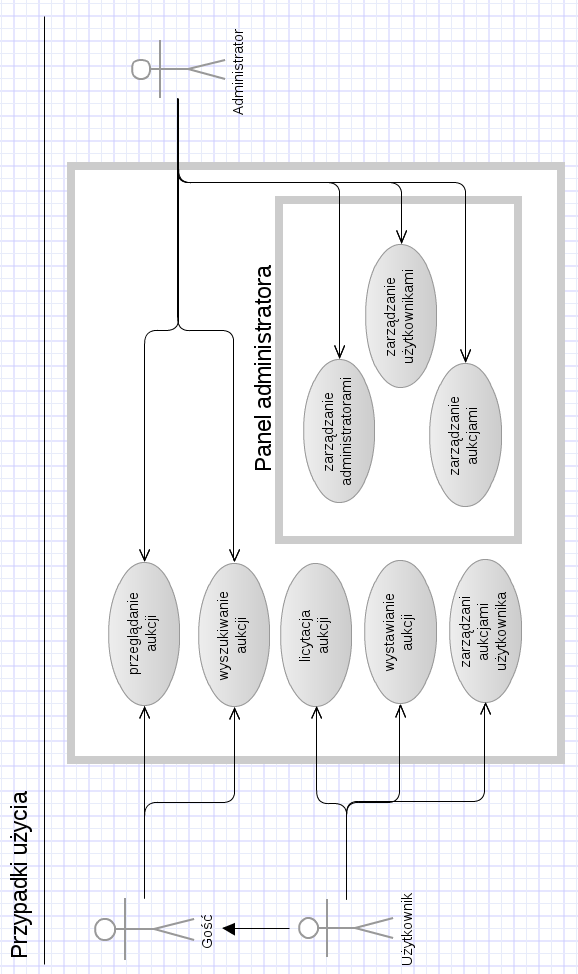
\includegraphics[height=0.8\textheight]{obrazki/usecase.png}
  \end{center}
  \caption{Diagram UML obrazujący przypadki użycia oraz aktorów.}
  \label{usecase}
\end{figure}

Wszystkie wyżej wymienione przypadki użycia powinny być zaimplementowane i~przetestowane. W~tym celu tworzone są testy behawioralne przy użyciu narzędzia \texttt{cucumber}. Testy te~przyjmują formę scenariuszy dla konkretnych przypadków użycia.

\lstset{language=sh, caption=Przykładowy scenariusz opisujący proces rejestracji nowego użytkownika., basicstyle=\ttfamily\footnotesize, numbers=left, numberstyle=\footnotesize, captionpos=b, backgroundcolor=\color{LightGray}} \label{code.simpleruby}
\begin{lstlisting}
Scenario: Registering a user account
  Given I am on the home page
  And no emails have been sent
  When I follow "Sign up"
  And I fill in the following:
    | user_email                 | user@example.com |
    | user_password              | monkey           |
    | user_password_confirmation | monkey           |
  And I press "Sign up"
  Then "user@example.com" should receive an email
  When "user@example.com" opens the email
  Then I should see "Confirmation instructions" in the email subject
  And I should see "You can confirm your account through the link below" in the email body
  And I should see "Confirm my account" in the email body
  When I follow "Confirm my account" in the email
  And I should see "Sign out"
\end{lstlisting}

\newpage

\subsection{Zadania i~ich realizacja}

Zadania, które należało wykonać aby zaimplementować system \textit{auctioner}:

\begin{enumerate}
  \item inicjacja środowiska -- zainstalowanie niezbędnych narzędzi, konfiguracja środowiska oraz stworzenie nowego projektu Ruby~on~Rails;
  \item konfiguracja projektu Ruby~on~Rails -- podpięcie wtyczek (gem), ustawienia konfiguracyjne dla projektu, utworzenie repozytorium \textit{Git} projektu, wykonanie czynności mających na~celu przygotowanie projektu dla realizacji jego architektury i~funkcjonalności;
  \item przygotowanie aplikacji na~możliwość obsługi wielu wersji językowych;
  \item utworzenie modeli użytkowników i~administratorów -- utworzenie schematu tabeli w~bazie danych, implementacja klas opakowujących, utworzenie prostych kontrolerów zarządzających modelami;
  \item dodanie funkcjonalności rejestracji/logowania -- podpięcie systemu autentykacji do istniejących modeli użytkownika i~administratora, utworzenie widoków dla funkcjonalności rejestracji, logowania, przypomnienia hasła, aktywacji konta oraz przygotowanie wersji językowych dla funkcjonalności;
  \item utworzenie modelu dla aukcji -- przygotowanie schematu dla bazy danych, utworzenie zależności pomiędzy modelami aukcji i użytkownika, utworzenie kontrolerów zarządzających aukcjami, utworzenie widoków dla aukcji, utworzenie ścieżek wywołań;
  \item dodanie możliwości wyszukiwania -- implementacja systemu zapytań do~bazy danych, obsługa tworzonych kwerend;
  \item utworzenie systemu publikacji i~podbijania aukcji -- dodanie maszyny stanów dla modelu aukcji, implementacja kontrolerów zarządzających zmianami stanu, zmiany w widokach dla funkcjonalności;
\end{enumerate}

\lstset{language=sh, caption=Lista zadań w~aplikacji \textit{ticgit}., basicstyle=\ttfamily\footnotesize, numbers=left, numberstyle=\footnotesize, captionpos=b, backgroundcolor=\color{LightGray}} \label{code.simpleruby}
\begin{lstlisting}
TicId  Title                        State   Date  Assgn    Tags
------------------------------------------------------------------------
69418c Create a new rails projec... reso... 11/07 placek   environment
36ce13 Prepare L10n and I18n env... reso... 11/07 placek   environment
fca367 Prepare a devise models f... reso... 11/07 placek   users
ed753d Create model for auction;... reso... 11/07 placek
b2296e Prepare a publication sys... reso... 11/07 placek   auction,state
\end{lstlisting}


\section{Projekt \textit{auctioneer}}

Poniżej zaprezentowano rezultat pracy nad projektem \textit{auctioneer}.

\subsection{Architektura}

Aplikacje pisane przy użyciu aplikacji szkieletowej Ruby~on~Rails opierają się na~architekturze \textit{MVC} (ang.~\textit{model-view-controller}). Oznacza to, że~w~aplikacji takiej wyróżnione są~warstwy odpowiedzialne za~dostęp do~danych i~ich ,,obróbkę'', realizację logiki biznesowej aplikacji oraz prezentację (interfejs graficzny).

\subsubsection{Warstwa danych -- model}

Ruby~on~Rails wykorzystuje moduł \texttt{ActiveRecord} do~opakowania rekordów, pochodzących z~relacyjnych baz danych, odpowiadającymi im obiektami. Dzięki temu programista może traktować tabele bazy danych jako klasę, a~rekordy tej tabeli jako jej instancje.

\begin{itemize}
  \item[admins]\hfill\\ reprezentacja danych modelu administratora; zawiera adres e-mail, zaszyfrowane hasło, stemple czasu (utworzenie i edycja rekordu) oraz dane logowania (stempel czasu, adres IP, z~którego się zalogowano),
  \item[users]\hfill\\ reprezentacja danych modelu użytkownika; zwiera adres e-mail, zaszyfrowane hasło, stemple czasu, dane logowania oraz dane aktywacji konta,
  \item[auctions]\hfill\\ reprezentacja danych modelu aukcji; zawiera tytuł, opis, cenę minimalną i~aktualną aukcji, aktualny stan, klucze (identyfikatory) użytkownika-właściciela i~użytkownika-zwycięzcy oraz stemple czasu.
\end{itemize}

Na~rysunku \ref{database} zamieszczono schemat tabeli bazy danych projektu \textit{auctioneer}. Listingi \ref{code.auction}, \ref{code.admin}, \ref{code.user} pokazują klasy opakowujące dane dla modeli projektu \textit{auctioneer}.

\begin{figure}[h]
\centering
\fbox{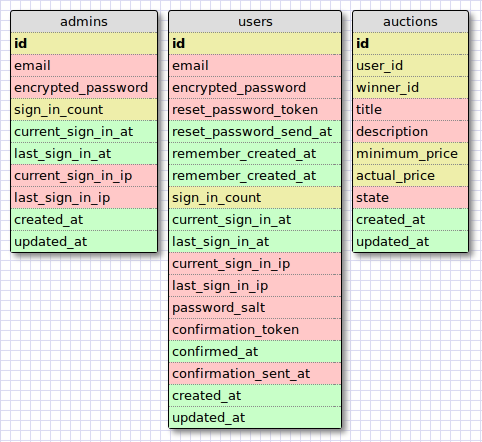
\includegraphics[width=0.6\textwidth]{obrazki/entity.png}}
\caption{Schemat bazy danych projektu \textit{auctioneer}}
\label{database}
\end{figure}

\lstset{language=Ruby, caption=Klasa reprezentacji modelu aukcji, basicstyle=\ttfamily\footnotesize, numbers=left, numberstyle=\footnotesize, captionpos=b, backgroundcolor=\color{LightGray}}
\begin{lstlisting}[label={code.auction}]
class Auction < ActiveRecord::Base
  EXPIRATION_AFTER = 7.days

  belongs_to :user
  belongs_to :winner, class_name: 'User'
  validates :title, presence: true
  validates :minimum_price, presence: true

  scope :created, where(state: :new)
  scope :public, where(state: :public)
  scope :closed, where(state: :closed)
  scope :won, where(state: :won)
  scope :finished, where('state = "closed" OR state = "won"')
  scope :won_by, ->(user) { where(state: :won).where(winner_id: user.id) }

  def self.about_to_finish
    time = Time.now
    now = Time.new(time.year, time.month, time.day, time.hour, 0)
    where(state: :public).
    where('created_at < ?', now - EXPIRATION_AFTER + 1.hour).
    where('created_at >= ?', now - EXPIRATION_AFTER)
  end

  # scope used in search engine
  def self.search(query)
    if query
      phrase = "%#{query}%"
      where('(title LIKE ?) OR (description LIKE ?)', phrase, phrase)
    else
      scoped
    end
  end

  # closing every expired auction
  def self.close_auctions
    self.about_to_finish.each do |auction|
      auction.close if auction.winner.nil?
      auction.win if auction.winner.present?
    end
  end

  state_machine initial: :new do
    after_transition any => :public do |auction, transition|
      auction.actual_price = auction.minimum_price
      auction.save!
    end

    event :publish do
      transition new: :public, if: ->(auction) {
        auction.description.present?
      }
    end

    event :close do
      transition public: :closed
    end

    event :win do
      transition public: :won, if: ->(auction) {
        auction.actual_price != auction.minimum_price && auction.winner.present?
      }
    end

    event :republish do
      transition closed: :public
    end
  end

end
\end{lstlisting}

\lstset{language=Ruby, caption=Klasa reprezentacji modelu administratora, basicstyle=\ttfamily\footnotesize, numbers=left, numberstyle=\footnotesize, captionpos=b, backgroundcolor=\color{LightGray}}
\begin{lstlisting}[label={code.admin}]
class Admin < ActiveRecord::Base
  devise :database_authenticatable, :trackable, :validatable,
         :timeoutable
  attr_accessible :email, :password, :password_confirmation
  validates_presence_of :email
  validates_uniqueness_of :email, case_sensitive: false

  scope :email_like, ->(email) { where('admins.email like ?', email) }
end
\end{lstlisting}

\lstset{language=Ruby, caption=Klasa reprezentacji modelu użytkownika, basicstyle=\ttfamily\footnotesize, numbers=left, numberstyle=\footnotesize, captionpos=b, backgroundcolor=\color{LightGray}}
\begin{lstlisting}[label={code.user}]
class User < ActiveRecord::Base
  devise :database_authenticatable, :registerable, :recoverable,
         :rememberable, :trackable, :validatable, :confirmable
  attr_accessible :email, :password, :password_confirmation,
         :remember_me
  validates_presence_of :email
  validates_uniqueness_of :email, case_sensitive: false
  has_many :auctions

  scope :email_like, ->(email) { where('users.email like ?', email) }
end
\end{lstlisting}

\subsubsection{Warstwa logiki -- kontroler}

\textit{Kontroler} jest elementem decyzyjnym realizującym założenia logiki biznesowej projektu. W~Ruby~on~Rails kontrolerami są~pewne klasy, które grupują w~sobie metody (tak zwane akcje). Akcje są~wykonywane podczas każdego zapytania HTTP. O~tym, która akcja zostanie wykonana, decyduje system rozpoznawania ścieżek i~parametrów zapytania -- \texttt{routes}. Listing \ref{code.controller} prezentuje przykładowy kontroler dla aplikacji \textit{auctioneer}.

\lstset{language=Ruby, caption=Przykładowy kontroler \texttt{Admin::UsersController} odpowiadający za~akcje związane z~zarządzaniem użytkownikami w panelu administratora, basicstyle=\ttfamily\footnotesize, numbers=left, numberstyle=\footnotesize, captionpos=b, backgroundcolor=\color{LightGray}}
\begin{lstlisting}[label={code.controller}]
class Admin::UsersController < ApplicationController
  before_filter :authenticate_admin!
  layout 'admin'

  def index
    @users = User.email_like(params[:like] || '%').paginate(page: params[:page])
  end

  def destroy
    @user = User.find(params[:id]).destroy
    flash[:notice] = t('admin.registrations.destroy')
    redirect_to admin_users_path
  end

  def login
    sign_in(:user, User.find(params[:id]))
    redirect_to root_path
  end

  def confirm
    User.find(params[:id]).confirm!
    redirect_to admin_users_path
  end
end
\end{lstlisting}

\subsubsection{Warstwa prezentacji -- widok}

Widoki to~szablony, generujące rezultaty -- odpowiedzi na~zadane zapytania protokołu HTTP. Są one wynikiem działania akcji kontrolera. W~aplikacji \textit{auctioneer} użyto metajęzyka \texttt{haml} do~tworzenia takich szablonów. Listing \ref{code.view} przedstawia przykładowy szablon widoku.

\lstset{language=Ruby, caption=Przykładowy widok -- lista użytkowników w~panelu administratora, basicstyle=\ttfamily\footnotesize, numbers=left, numberstyle=\footnotesize, captionpos=b, backgroundcolor=\color{LightGray}}
\begin{lstlisting}[label={code.view}]
= form_tag admin_users_path, method: :get do
  = label_tag :email, "Filter by email:"
  = text_field_tag :like, h(params[:email])
  = submit_tag "Filter"
  .grey
    use '%' to match anything (like '%examp%')

- unless params[:like].nil?
  %p
    Filtered with
    %strong
      = h(params[:like])

= will_paginate(@users)

%table
  %tr
    %th Email
    %th Created at
    %th Confirmed at
    %th Last signed in
    %th Sign in IP
    %th{ colspan: 2 } Actions
  - @users.each do |user|
    %tr
      %td= user.email
      %td= user.created_at
      %td= user.confirmed_at.present? ? user.confirmed_at : 'not confirmed yet'
      %td= user.last_sign_in_at.present? ? user.last_sign_in_at : 'not signed in yet'
      %td= user.last_sign_in_at.present? ? user.last_sign_in_ip : 'not signed in yet'

      - if user.confirmed?
        %td= link_to 'Sign in', admin_user_login_path(user)
      - else
        %td= link_to 'Confirm', admin_user_confirm_path(user)
      %td= link_to 'Delete', admin_user_delete_path(user), confirm: 'Are you sure?'

= will_paginate(@users)
\end{lstlisting}

\subsection{Testy}

W~realizacji poszczególnych funkcjonalności systemu ważną rolę spełniają testy. Stanowią one potwierdzenie poprawnego działania poszczególnych komponentów, a także chronią programistę przed popełnieniem nie przewidzianego błędu.

\subsubsection{Testy jednostkowe}

Testy jednostkowe \texttt{rspec} sprawdzają poprawność działania elementów logiki biznesowej, metod pomocniczych dla warstwy danych i~widoku oraz reakcji na zapytania HTTP. Testy jednostkowe znajdują się w~katalogu \texttt{spec}. Po~wywołaniu komendy \verb+rake spec+ aplikacja zostaje przetestowana. Wyniki takiego testowania zawiera listing \ref{code.spec}.

\lstset{language=Ruby, caption=Wyniki testowania aplikacji narzędziem \texttt{rspec}, basicstyle=\ttfamily\footnotesize, numbers=left, numberstyle=\footnotesize, captionpos=b, backgroundcolor=\color{LightGray}}
\begin{lstlisting}[label={code.spec}]
$ rake spec
ApplicationController
  routing
    routes to static_admin/admins#dashboard
    routes to static_admin/admins#index
    routes to static_admin/users#index
    routes to static_static_pages#landing

AuctionsController
  routing
    routes to #index
    routes to #show
    routes to #new
    routes to #edit
    routes to #create
    routes to #update
    routes to #destroy

Auction
  about_to_finish
    should not be empty
  about_to_finish
    should be empty
  about_to_finish
    should be empty
  close_auctions
    should eq 1

AdminHelper
  total_count_of
    should return a quantity of all records in model

AuctionsHelper
  short_description
    should return a shorten text with no html tags and ended with '...'

ApplicationHelper
  after_sign_in_path_for
    should return a proper url

Finished in 6.98 seconds
18 examples, 0 failures
\end{lstlisting}

\subsubsection{Testy behawioralne}

Testy behawioralne sprawdzają zachowanie aplikacji przy zadanych warunkach. W~projektach Ruby~on~Rails zwykle używa się w~tym celu narzędzia \textit{cucumber}. Testy takie składają się z~tak zwanych scenariuszy. Scenariusz to~lista kroków, w~których realizowane są poszczególne działania w~aplikacji oraz sprawdzane założenia. Testy behawioralne wraz z~konfiguracją środowiska testującego znajdują się w~katalogu \texttt{features}. Po~wywołaniu komendy \verb+rake cucumber+ aplikacja zostaje przetestowana. Wyniki takiego testowania zawiera listing \ref{code.cukes}.

\lstset{language=Ruby, caption=Przykładowy scenariusz opisujący system rejestracji i~logowania użytkowników, basicstyle=\ttfamily\footnotesize, numbers=left, numberstyle=\footnotesize, captionpos=b, backgroundcolor=\color{LightGray}}
\begin{lstlisting}[label={code.cukes}]
Feature: User accounts
  In order to have a private account
  A user
  Wants to manage it

  Scenario: Registering a user account
    Given I am on the home page
    And no emails have been sent
    When I follow "Sign up"
    And I fill in the following:
      | user_email                 | user@example.com |
      | user_password              | monkey           |
      | user_password_confirmation | monkey           |
    And I press "Sign up"
    Then "user@example.com" should receive an email
    When "user@example.com" opens the email
    Then I should see "Confirmation instructions" in the email subject
    And I should see "You can confirm your account" in the email body
    And I should see "Confirm my account" in the email body
    When I follow "Confirm my account" in the email
    And I should see "Sign out"

  Scenario: Changing users password
    Given a user "quentin"
    And I am on the home page
    When I follow "Sign in"
    And I follow "Forgot your password?"
    And I fill in the following:
      | user_email | quentin@example.com |
    And I press "Send me reset password instructions"
    Then I should see "You will receive an email with instructions"
    And "quentin@example.com" should receive an email
    When "quentin@example.com" opens the email
    Then I should see "Reset password instructions" in the email subject
    And I should see "link to change your password" in the email body
    When I follow "Change my password" in the email
    Then I should see "Change your password"
    When I fill in the following:
      | user_password              | monkey |
      | user_password_confirmation | monkey |
    And I press "Change my password"

  Scenario: Resend a confirmation instructions
    Given I am on the home page
    And an unconfirmed user "user"
    And a clear email queue
    When I follow "Sign up"
    And I follow "Didn't receive confirmation instructions?"
    Then I should see "Resend confirmation instructions"
    When I fill in the following:
      | user_email | user@example.com |
    And I press "Resend confirmation instructions"
    Then I should see "You will receive an email with instructions"
    And "user@example.com" should receive an email
    When "user@example.com" opens the email
    Then I should see "Confirmation instructions" in the email subject
    And I should see "You can confirm your account" in the email body

  Scenario: Logging in and out
    Given a user "quentin"
    And I am on the home page
    When I follow "Sign in"
    And I fill in the following:
      | user_email    | quentin@example.com |
      | user_password | secret              |
   And I press "Sign in"
   Then I should see "quentin@example.com"
\end{lstlisting}

\subsection{Dziennik realizacji zadań}

Realizacja poszczególnych zadań ma~swoje odzwierciedlenie w~historii kodu w~repozytorium \textit{Git}. Poniżej przedstawiono historię zmian kodu.

\begin{verbatim}
* 5f69148: changes in report; closed chapter describing application
* 1b8d6b1: changes in report; minor changes in application
* cf54641: removed ruby-debug from Gemfile
* 8c2da87: another changes due to report
* 99ba8ff: added new content to report; some small corrections
* d360dfa: fixed spec tests for auction model
* fd1c522: changes in report; added new chapter
* a2fb439: [#134409] added simple relancing system with hourly checking for winners
* 9eb16d9: [#8269df] ordering the search results by title, minimum and actual price
* 4707b6a: some more resolution to report
* f73219b: changes in report due to suggestions
* 9bd648b: [#378254] simple search engine added
* c5a3008: [#b2296e] auctions are treated as state machine
*   c9526a7: Merging branches
|\
| * 2c1e199: [#fca367 and #ed753d] simple schema of auctioning system
| * bcc6b5a: [#fca367] changes in admin and user models; prepared devise system
* | b234283: removed pdf file from documentation
* | 6ce2ac8: more specific documentation about used tools
* | 2972c55: some logical changes in report
* | 2017f51: added a doc directory containing a documentation
* | 8c8cb9a: [#fca367] added admin and user models;
|/
* 836ffa3: removed unnecesary README_FOR_APP file
* 17550e4: [#36ce13] added localization scopes
* f42d5dc: first commit; new project created; initialized gems
\end{verbatim}

\section{Podręcznik użytkownika}

Poniżej zamieszczono opis stworzonej aplikacji od~strony osoby jej użytkującej. Osobą taką może być jeden z~trzech aktorów: gość, zwykły użytkownik oraz administrator. Możliwe działania dla poszczególnych aktorów tworzą scenariusze dla poszczególnych przypadków użycia. Założono, że~punktem wyjścia jest odwiedzenie przez aktora strony głównej projektu (Rys. \ref{screen01}).

\begin{figure}[h]
\centering
\fbox{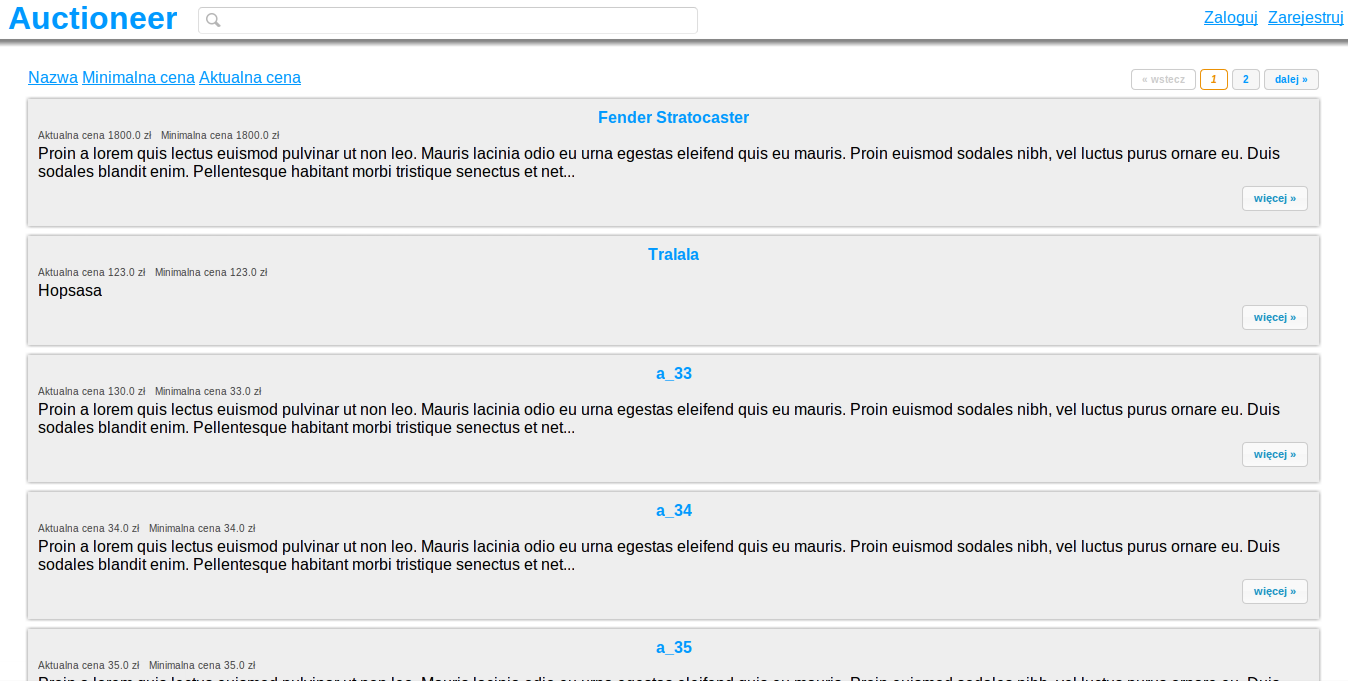
\includegraphics[width=\textwidth]{obrazki/auctioneer01.png}}
\caption{Strona główna serwisu \textit{auctioneer} -- lista wystawionych aukcji}
\label{screen01}
\end{figure}

\subsection{Opis projektu od strony gościa}

\paragraph{Strona główna}

Na~stronie głównej znajdują się następujące aktywne elementy:

\begin{itemize}
  \item pole tekstowe wyszukiwarki aukcji,
  \item link ,,Zaloguj'',
  \item link ,,Zarejestruj'',
  \item link ,,Nazwa'',
  \item link ,,Minimalna cena'',
  \item link ,,Aktualna cena'',
  \item zestaw przycisków: ,,wstecz'', ,,1'', ,,2'', \ldots, ,,dalej'',
  \item lista aukcji,
  \item link-nagłówek ,,Auctioneer''.
\end{itemize}

Pole tekstowe wyszukiwarki aukcji pozwala na~wyselekcjonowanie aukcji, znajdujących się w~liście poniżej, według zadanych kryteriów. Wpisanie wyszukiwanej frazy oraz~wciśnięcie klawisza \texttt{Enter} spowoduje przejście do~strony z~wynikami wyszukiwania (Rys. \ref{screen02}). Strona z~wynikami wyszukiwania jest podobna do~strony głównej, z~tą~różnicą, że~ponad wynikami wyszukiwania widoczna jest informacja na~temat wyszukiwanej frazy.

\begin{figure}[h]
\centering
\fbox{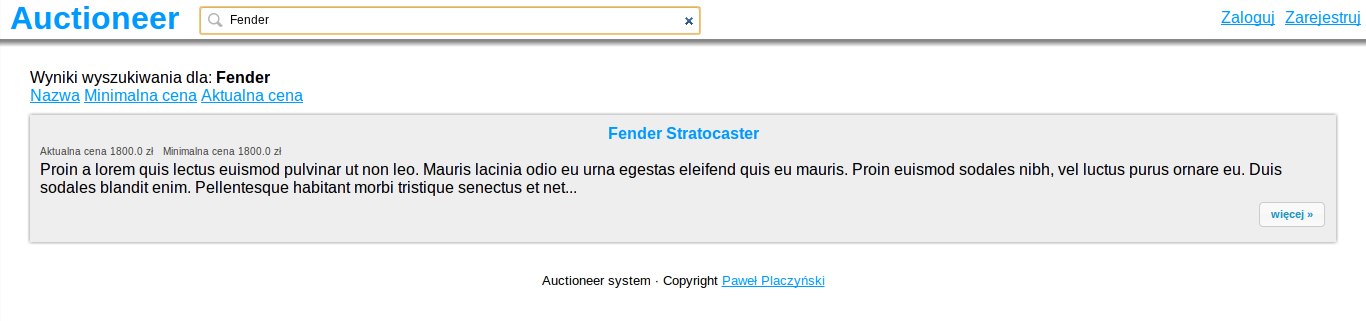
\includegraphics[width=\textwidth]{obrazki/auctioneer02.png}}
\caption{Działanie wyszukiwarki aukcji serwisu \textit{auctioneer}}
\label{screen02}
\end{figure}

Link ,,Zaloguj'' przekierowuje gościa do~formularza logowania (Rys. \ref{screen03}). Formularz logowania opisany został poniżej. Link ,,Zarejestruj'' przekierowuje do~formularza rejestracji (Rys. \ref{screen13}). Zestaw odsyłaczy: ,,Nazwa'', ,,Minimalna cena'' oraz ,,Aktualna cena''  zmienia kolejność wyświetlania aukcji, sortując je~według nazwy, minimalnej oraz aktualnej ceny (ponowne wybranie linku odwraca kolejność sortowania). Link-nagłówek ,,Auctioneer'' prowadzi zawsze na~stronę główną.

\begin{figure}[h]
\centering
\fbox{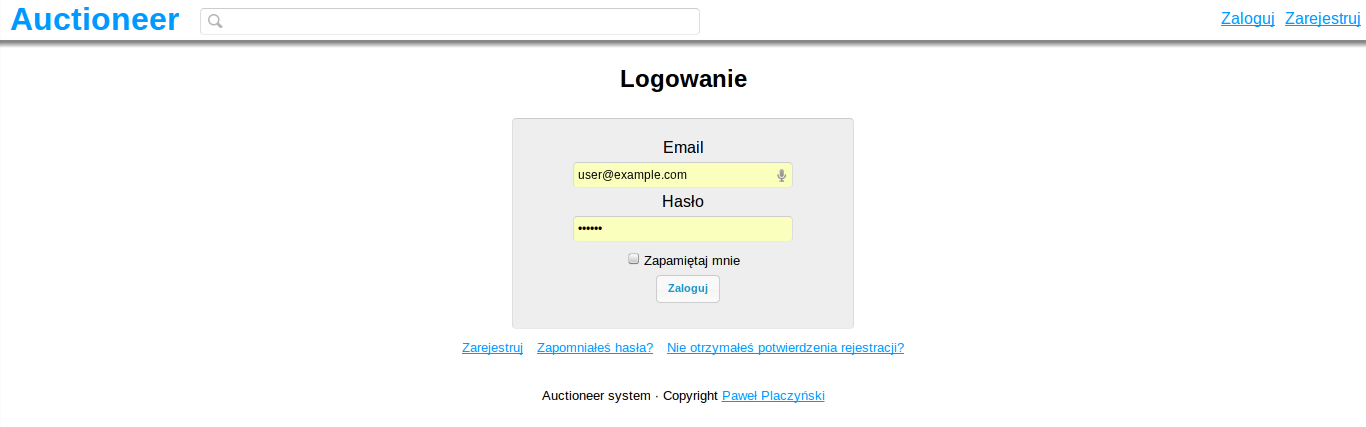
\includegraphics[width=\textwidth]{obrazki/auctioneer03.png}}
\caption{Ekran logowania}
\label{screen03}
\end{figure}

\begin{figure}[h]
\centering
\fbox{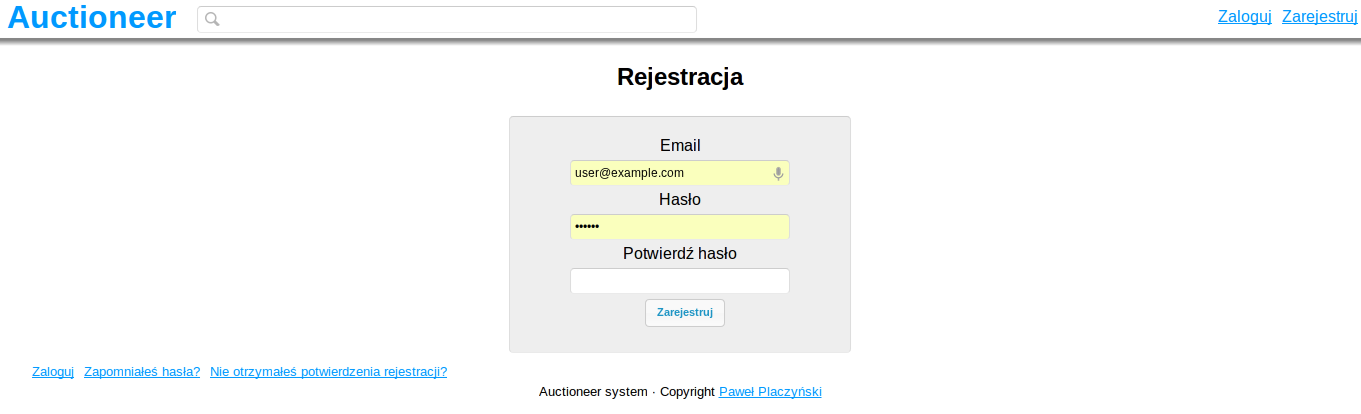
\includegraphics[width=\textwidth]{obrazki/auctioneer13.png}}
\caption{Ekran rejestracji}
\label{screen13}
\end{figure}

Zestaw przycisków: ,,Wstecz'', ,,1'', ,,2'', \ldots, ,,Dalej'' pozwala przeglądać kolejne strony wystawionych aukcji (mechanizm ,,paginacji stron'').


\paragraph{Aukcje}

Na stronie głównej znajduje się lista aukcji. Każda aukcja ma~przy swoim opisie przycisk ,,Więcej'' prowadzący do~strony aukcji (Rys. \ref{screen09} oraz Rys. \ref{screen05}).

\begin{figure}[h]
\centering
\fbox{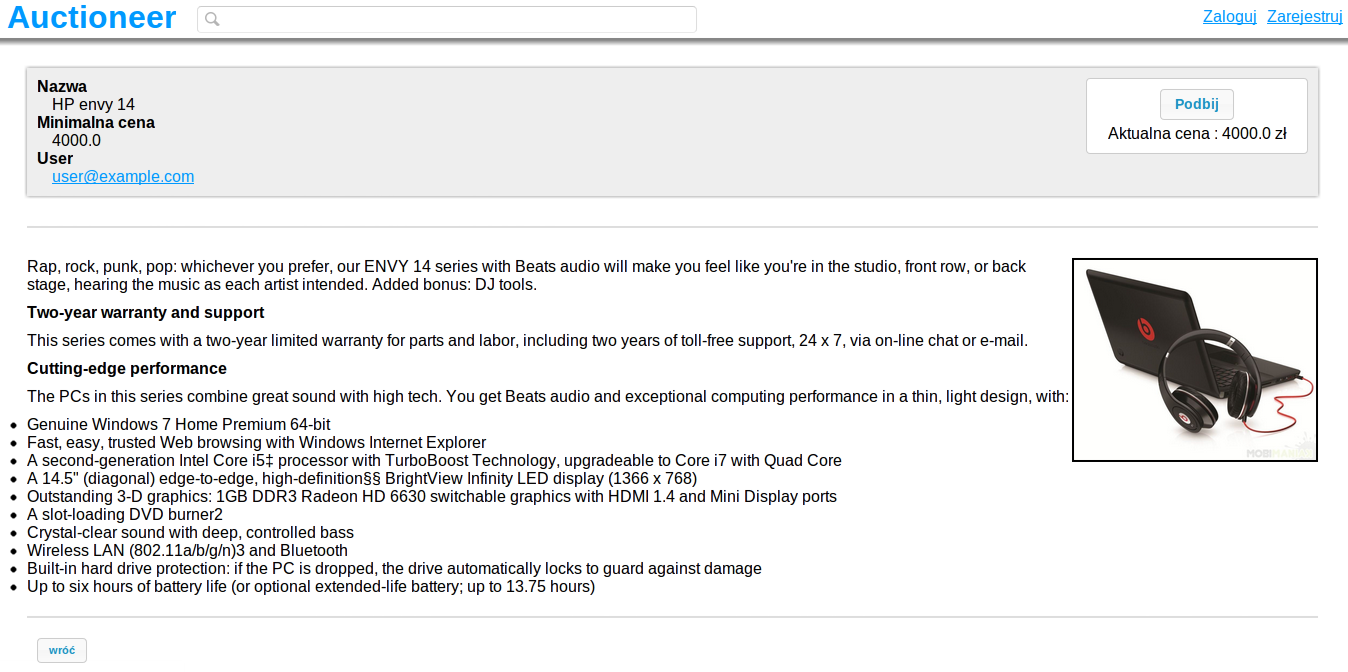
\includegraphics[width=\textwidth]{obrazki/auctioneer09.png}}
\caption{Strona aukcji zawierająca detale. Widok dla gościa lub zalogowanego użytkownika nie wystawiającego aukcję}
\label{screen09}
\end{figure}

\begin{figure}[h]
\centering
\fbox{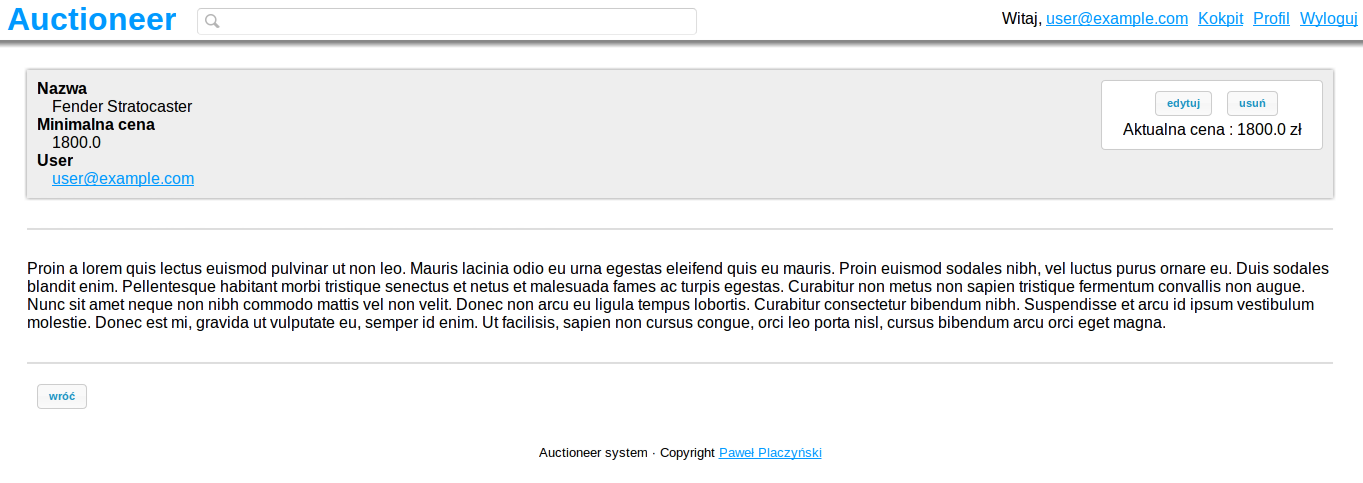
\includegraphics[width=\textwidth]{obrazki/auctioneer05.png}}
\caption{Strona aukcji zawierająca detale. Widok dla zalogowanego użytkownika wystawiającego aukcję}
\label{screen05}
\end{figure}

Strona aukcji zawiera pełny opis wystawionej aukcji. Przycisk ,,Wróć'' pozwala wrócić na~stronę główną, a przycisk ,,Podbij'' prowadzi do~formularza podbijania aukcji (Rys. \ref{screen10}). Jeśli użytkownik nie jest zalogowany to~po~naciśnięciu przycisku ,,Podbij'' zostaje on~przekierowany do~formularza logowania. Po~prawidłowym zalogowaniu, użytkownik zostaje automatycznie przekierowany do~formularza podbijania aukcji.

\begin{figure}[h]
\centering
\fbox{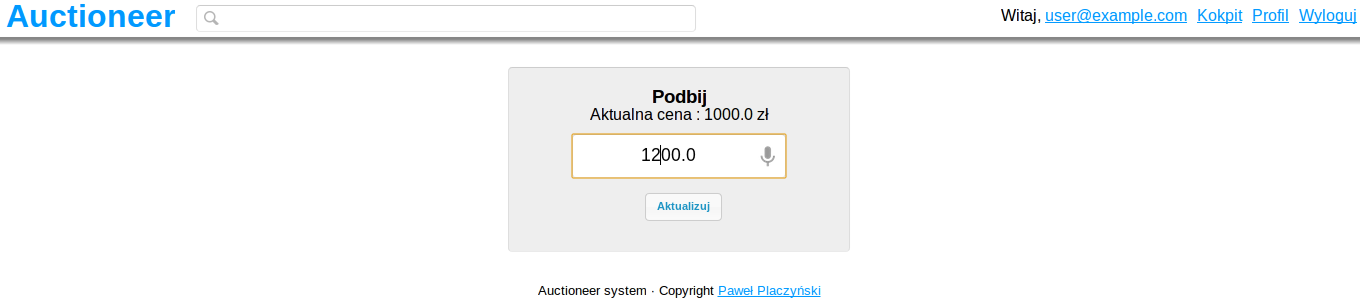
\includegraphics[width=\textwidth]{obrazki/auctioneer10.png}}
\caption{Formularz podbijania aukcji}
\label{screen10}
\end{figure}

\paragraph{Formularz logowania}

Formularz logowania umożliwia niezalogowanemu użytkownikowi otworzyć nową, bezpieczną sesję. Pola tekstowe pozwalają na~wprowadzenie danych logowania: adresu e-mail oraz hasła. Użycie opcji ,,Zapamiętaj mnie'' skutkuje tym, że~sesja użytkownika nie wygaśnie, gdy użytkownik będzie nieaktywny przez dłuższy czas. Przycisk ,,Zaloguj'' służy do~zatwierdzenia operacji logowania.


Jeżeli operacja logowania przeszła pomyślnie (użytkownik o~podanym adresie e-mail oraz haśle posiada konto w~serwisie oraz~zostało aktywowane, ponadto adres e-mail oraz hasło zostały poprawnie podane), to~otwarta zostaje sesja użytkownika oraz zostanie on~przekierowany do~panelu użytkownika. Akcje dla zalogowanego użytkownika opisuje podrozdział \ref{man.user}.

Pod formularzem znajdują się odnośniki pomagające użytkownikowi zarejestrować się, bądź odzyskać utracone hasło. Link ,,Zarejestruj'' przekierowuje do~formularza rejestracji, link ,,Zapomniałeś hasła?'' przekierowuje do~formularza zmiany hasła (Rys. \ref{screen11}), natomiast link ,,Nie otrzymałeś potwierdzenia rejestracji?'' przekierowuje do~formularza ponownego wysłania potwierdzenia rejestracji, gdy takie potwierdzenie nie zostało poprawnie wysłane na~adres e-mail użytkownika (Rys. \ref{screen12}).

\begin{figure}[h]
\centering
\fbox{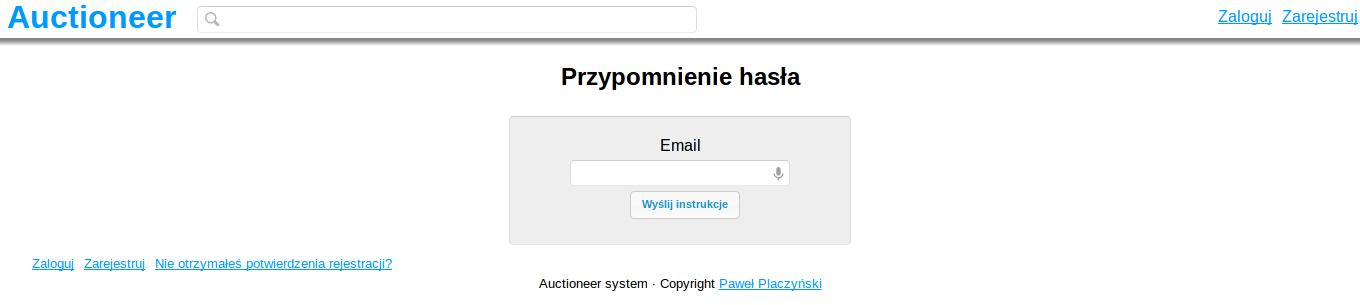
\includegraphics[width=\textwidth]{obrazki/auctioneer11.png}}
\caption{Formularz przypomnienia hasła}
\label{screen11}
\end{figure}

\begin{figure}[h]
\centering
\fbox{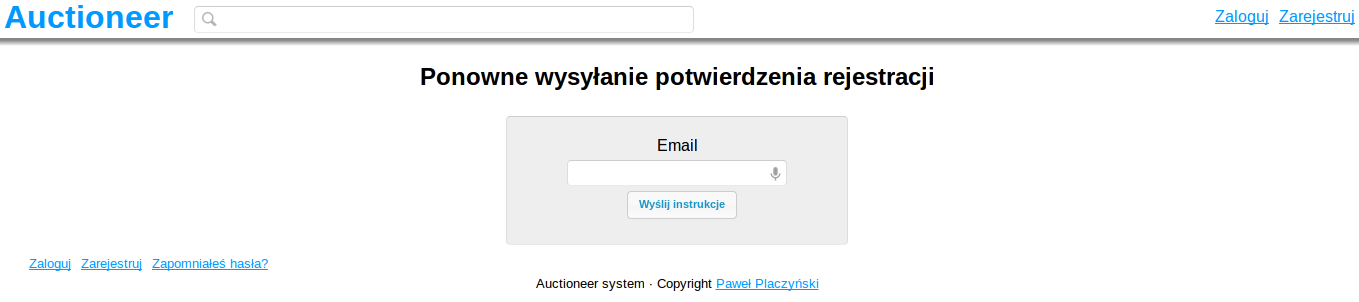
\includegraphics[width=\textwidth]{obrazki/auctioneer12.png}}
\caption{Formularz ponownego wysłania potwierdzenia rejestracji}
\label{screen12}
\end{figure}

\subsection{Opis projektu od~strony użytkownika} \label{man.user}

\paragraph{Panel użytkownika (Kokpit)}

Po~zalogowaniu, użytkownik zostaje przekierowany do~panelu użytkownika (Rys. \ref{screen04}). W~,,nagłówku'' strony znajduje się zestaw odnośników: link ,,Kokpit'' prowadzi do~panelu użytkownika, link ,,Profil'' prowadzi do~formularza edycji profilu (Rys. \ref{screen07}), a~link ,,Wyloguj'' zamyka sesję użytkownika i~przekierowuje na~stronę główną.

\begin{figure}[h]
\centering
\fbox{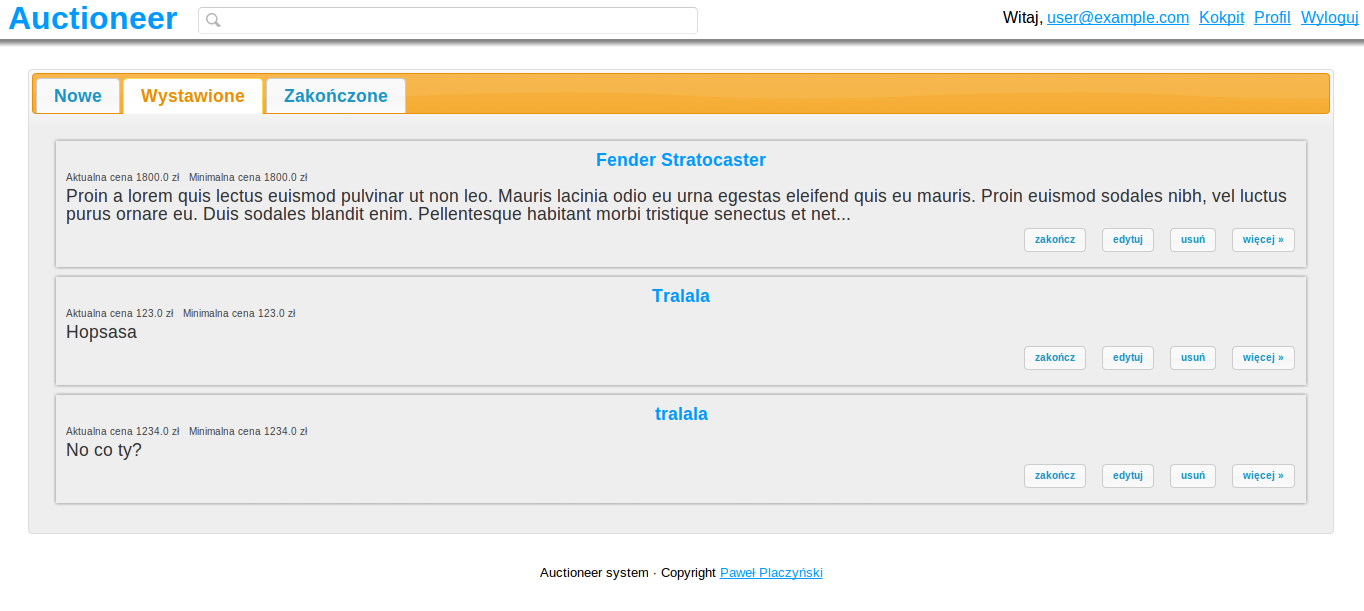
\includegraphics[width=\textwidth]{obrazki/auctioneer04.png}}
\caption{Kokpit użytkownika wraz z~listami aukcji użytkownika}
\label{screen04}
\end{figure}

\begin{figure}[h]
\centering
\fbox{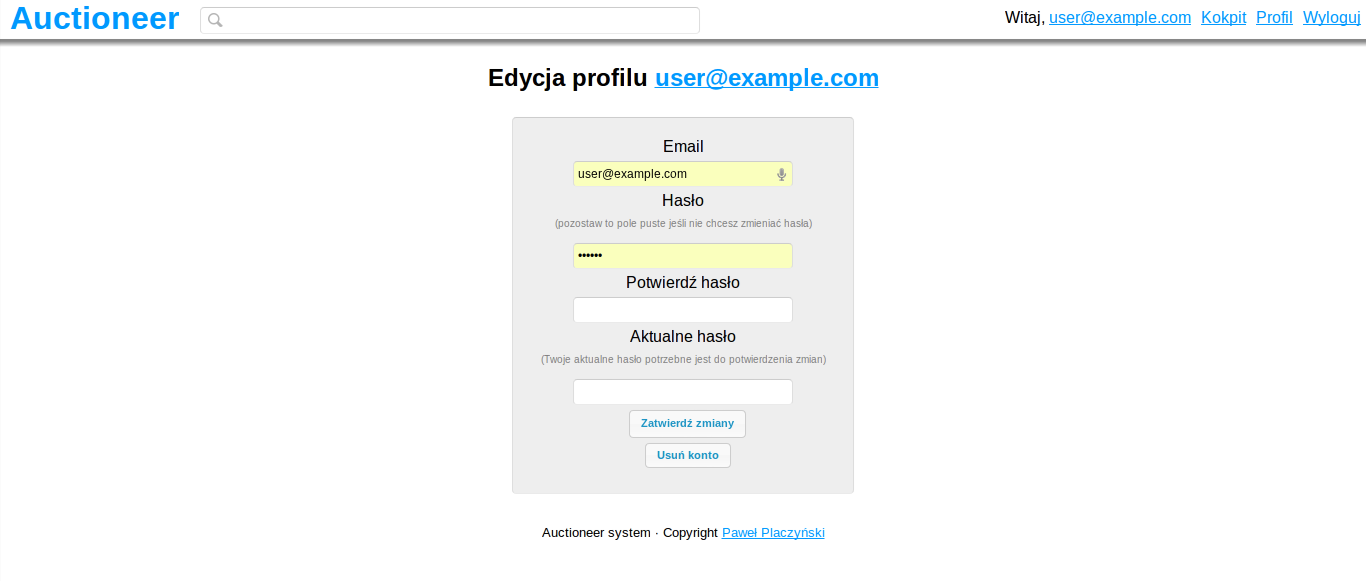
\includegraphics[width=\textwidth]{obrazki/auctioneer07.png}}
\caption{Panel edycji profilu użytkownika}
\label{screen07}
\end{figure}

Na~panelu użytkownika widoczne są zakładki: \textit{Nowe}, \textit{Wystawione}, \textit{Zakończone}, \textit{Wygrane}. Otwierają one kolejno: listę nowo utworzonych aukcji użytkownika, listę aukcji aktualnie wystawionych przez użytkownika, listę aukcji zakończonych oraz listę aukcji wygranych przez użytkownika.


Każda aukcja, z~dowolnej, wyżej wymienionej listy, posiada dwa przyciski: ,,edytuj'' -- prowadzący do~formularza edycji aukcji (Rys. \ref{screen06}) oraz ,,usuń'' -- powodujący usunięcie aukcji po~uprzednim potwierdzeniu operacji. Ponadto aukcja posiada przyciski zmiany stanu: aukcje z~listy \textit{Nowe} posiadają przycisk ,,wystaw'', aukcje z~listy \textit{Wystawione} -- ,,zakończ'' oraz~aukcje z~listy \textit{Zakończone} -- ,,wystaw ponownie''.

\begin{figure}[h]
\centering
\fbox{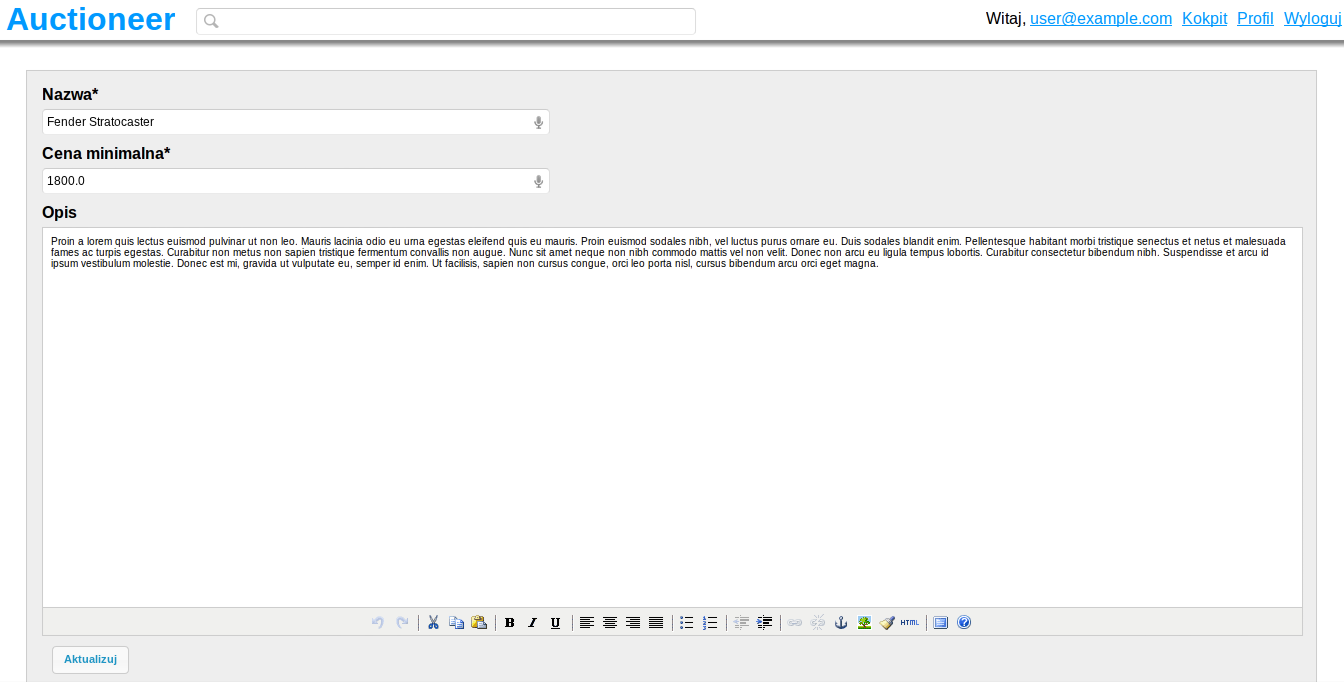
\includegraphics[width=\textwidth]{obrazki/auctioneer06.png}}
\caption{Panel edycji aukcji}
\label{screen06}
\end{figure}

\paragraph{Panel edycji aukcji}

Panel edycji aukcji posiada pole tekstowe zmiany nazwy (tytułu) aukcji, pole tekstowe zmiany ceny minimalnej aukcji oraz pole tekstowe zaopatrzone w~zestaw narzędzi, służących do~formatowania tekstu, do~edycji opisu aukcji. Przycisk ,,Aktualizuj'' zatwierdza zmiany.

\subsection{Opis projektu od strony administratora}

Aby odwiedzić panel administratora (Rys. \ref{screen08}) należy podać ścieżkę \textit{adres\_bazowy\_aplikacji}\texttt{/admin}. Wyświetli się wówczas formularz logowania administratora. Podając odpowiednie dane (adres e-mail oraz hasło) można zarządzać aplikacją z~poziomu administratora.

\begin{figure}[h]
\centering
\fbox{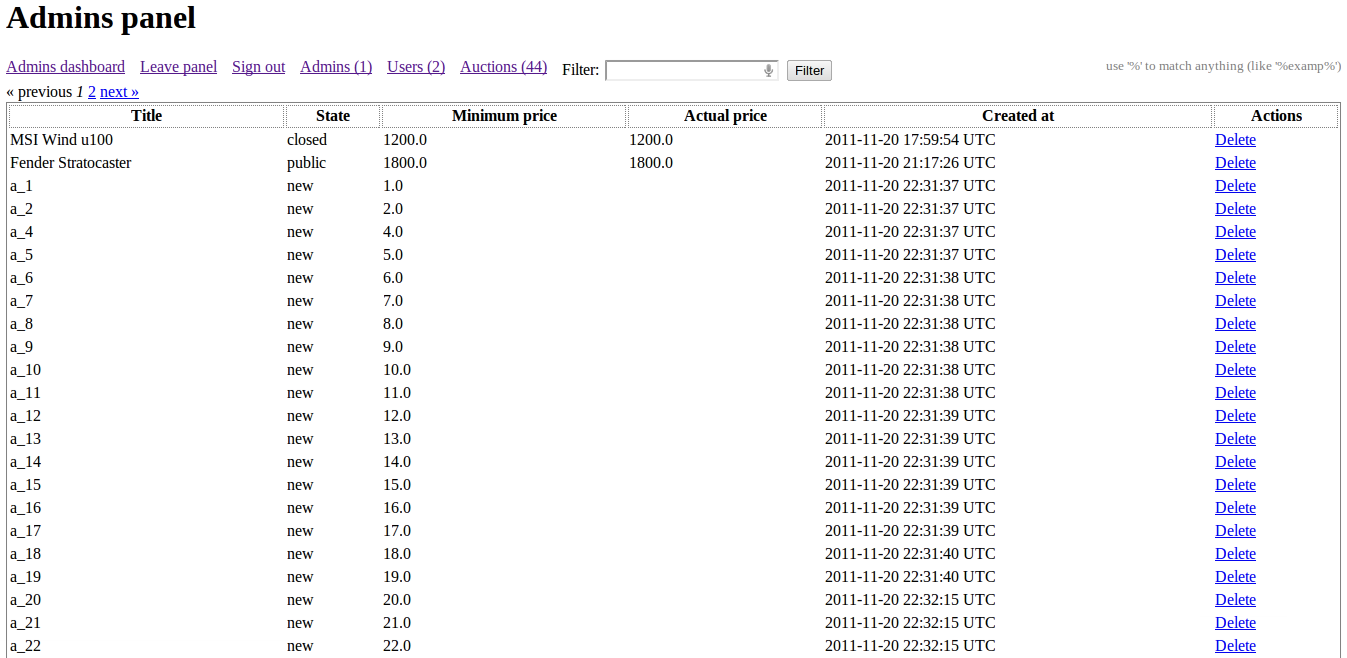
\includegraphics[width=\textwidth]{obrazki/auctioneer08.png}}
\caption{Panel administratora z~listą aukcji}
\label{screen08}
\end{figure}

W~panelu administratora znajdują się:

\begin{itemize}
  \item Link ,,Leave panel'', który pozwala wyjść z~panelu, pozostając zalogowanym jako administrator. Link ten przekierowuje na~stronę główną.
  \item Link ,,Sign out'' umożliwia wylogowanie administratora.
  \item Link ,,Admins'' pokazuje listę administratorów serwisu. Lista ta~udostępnia następujące akcje: wyszukanie administratora według adresu e-mail (pole tekstowe oznaczone etykietą ,,Filter'') oraz usunięcie administratora (link ,,Delete'', przy czym nie jest możliwe usunięcie aktualnie zalogowanego administratora).
  \item Link ,,Users'' pokazuje listę użytkowników. Lista ta~pozwala na~wyszukanie użytkownika według adresu e-mail (pole tekstowe oznaczone etykietą ,,Filter''), usunięcie użytkownika (link ,,Delete'') oraz zalogowanie się jako użytkownik (link ,,Login'').
  \item Link ,,Auctions'' pokazuje listę aukcji. Lista pozwala na~wyszukanie aukcji według tytułu lub opisu aukcji (pole tekstowe ,,Filter'') oraz usunięcie aukcji (link ,,Delete'').
\end{itemize}


\chapter{Podsumowanie}

Aplikacja szkieletowa Ruby~on~Rails ma~wiele zalet pozwalających na~pracę przy pomocy metodyki programowania zwinnego. Struktura aplikacji opartych na~frameworku Ruby~on~Rails jest przejrzysta, jasna i~zorganizowana. Kod takiej aplikacji jest czytelny, a~do~jego zrozumienia wystarczy znajomość języka angielskiego.


Ponadto ściśle wyodrębnione warstwy aplikacji pozwalają na~logiczny podział zadań poszczególnych komponentów oraz na~uniknięcie nadmiarowych bądź nieoczekiwanych operacji. Zapewnia to~bezpieczeństwo oraz dobrą kontrolę nad realizacją funkcjonalności.


Ruby~on~Rails posiada szereg wtyczek, dodatków, które realizują mniej lub bardziej skomplikowane działania. Można nimi w~prosty sposób zarządzać, co~sprawia, że~praca nad aplikacją jest prostsza i~bardziej efektywna.

\section{Obserwacje}

Podczas realizacji pracy poczyniono następujące obserwacje:

\begin{itemize}
  \item Język \textit{Ruby} ze względu na~swoją naturę umożliwia swobodne tworzenie dowolnego typu aplikacji. Możliwość wyboru pomiędzy programowaniem strukturalnym, obiektowym, funkcyjnym lub nawet metaprogramowaniem nie ogranicza programisty, a~wręcz pozwala mu~na~szybszą implementację założeń projektowych bez potrzeby zastanawiania się nad szczegółami.
  \item System zarządzania wtyczkami \textit{RubyGems} wraz z~pomocą narzędzia \texttt{bundler} zapewnia doskonałą kontrolę nad zależnościami projektu bez potrzeby troski o~instalację wtyczek.
  \item Ścisły podział aplikacji Ruby~on~Rails na~warstwy (model MVC) pozwala określić dokładnie zadania i~cele poszczególnych komponentów. Umożliwia to~lepszą kontrolę nad realizacją funkcjonalności oraz eliminację błędów mogących prowadzić do~poważnych usterek bezpieczeństwa danych biznesowych.
  \item Możliwość hierarchizacji komponentów warstwy logiki (kontrolerów) pomaga w~dobrej organizacji zakresu działań i~akcji przeprowadzanych przez użytkowników aplikacji na~danych.
  \item Podział warstwowy pozwala także zwiększyć czytelność kodu, co~znacznie przyspiesza i~usprawnia pracę nad nim.
  \item Interesujący system tworzenia kwerend modułu \texttt{ActiveRecord} pozwala na~szybkie i~czytelne konstruowanie zapytań bazy danych bez potrzeby konstruowania skomplikowanych kwerend w~języku \textit{SQL}. Pozwala to~także na~wykonywanie operacji na~bazie danych niezależnie od~systemu zarządzania bazą danych (DBMS).
  \item Testy jednostkowe i~behawioralne pozwalają szybko sprawdzić poprawność działania poszczególnych elementów aplikacji bez potrzeby jej uruchamiania, czy wdrażania.
  \item Narzędzie \texttt{cucumber} wspomaga współpracę z~potencjalnym klientem: scenariusze testujące funkcjonalność mogą być pisane przez programistę i~przez klienta. W~zasadzie tego typu scenariusze wraz z~szkicami (mockupami) stanowią pełną dokumentację przypadków użycia (a zatem funkcjonalności, założeń projektu).
  \item Symulacja pracy w~metodyce Scrum wyłania jasno określone cele, przez co~zadania są~szczegółowe oraz brak w~nich niedopowiedzeń.
  \item System kontroli wersji pozwala na~sprawną pracę nad projektem w~przypadkach częstych zmian w~projekcie. Jest on~dobrym narzędziem, wspomagającym pracę w~metodyce programowania zwinnego.
\end{itemize}


\listoffigures
\addcontentsline{toc}{chapter}{Spis rysunków}

\lstlistoflistings
\addcontentsline{toc}{chapter}{Spis listingów}

\begin{thebibliography}{99}

  \bibitem{ror} \emph{Strona domowa projektu Ruby~on~Rails} \url{http://rubyonrails.pl} (stan na~dzień \today)

  \bibitem{rspec} \emph{Narzędzie Rspec do testów jednostkowych i~funkcjonalnych} \url{http://rspec.info/} (stan na~dzień \today)

  \bibitem{cucumber} \emph{Narzędzie Cucumber pozwalające na wykonywanie testów behavioralnych} \url{http://cukes.info} (stan na~dzień \today)

  \bibitem{haml} \emph{Meta-język szablonów dokumentów XHTML} \url{http://haml-lang.com/} (stan na~dzień \today)

  \bibitem{sass} \emph{Meta-język szablonów dokumentów CSS} \url{http://sass-lang.com/} (stan na~dzień \today)

  \bibitem{devise} \emph{W~pełni konfigurowalny system autentyfikacji użytkowników dla Ruby~on~Rails} \url{https://github.com/plataformatec/devise} (stan na~dzień \today)

  \bibitem{will.paginate} \emph{Plugin paginacji stron dla Ruby~on~Rails} \url{https://github.com/mislav/will_paginate} (stan na~dzień \today)

  \bibitem{tiny.mce} \emph{Rozwinięty edytor HTML dla stron internetowych} \url{http://tinymce.moxiecode.com/} (stan na~dzień \today)

  \bibitem{sqlite3} \emph{Lekka i~szybka relacyjna baza danych SQL} \url{http://www.sqlite.org/} (stan na~dzień \today)

  \bibitem{jquery} \emph{Biblioteka programistyczna języka JavaScript} \url{http://docs.jquery.com/Main_Page} (stan na~dzień \today)

  \bibitem{git} \emph{System kontroli wersji Git} \url{http://git-scm.com} (stan na~dzień \today)

  \bibitem{ticgit} \emph{ticgit -- manager zadań projektowych dla projektów używających system kontroli wersji Git} \url{https://github.com/schacon/ticgit/wiki/} (stan na~dzień \today)

  \bibitem{ticgitweb} \emph{Webowy interfejs dla narzędzia ticgit -- ticgitweb} \url{https://github.com/schacon/ticgit/wiki/TicGitWeb} (stan na~dzień \today)

  \bibitem{zsh} \emph{Powłoka ZSH} \url{http://www.zsh.org/} (stan na~dzień \today)

  \bibitem{screen} \emph{GNU~screen} \url{http://www.gnu.org/software/screen/} (stan na~dzień \today)

  \bibitem{vim} \emph{Rozbudowany edytor tekstu Vim} \url{http://www.vim.org/} (stan na~dzień \today)

  \bibitem{rvm} \emph{System kontrolii wersji języka Ruby RVM} \url{https://rvm.beginrescueend.com/} (stan na~dzień \today)

  \bibitem{sqliteman} \emph{Sqliteman -- graficzne narzędzie do~zarządzania bazą danych Sqlite} \url{http://sqliteman.com/} (stan na~dzień \today)

  \bibitem{heroku} \emph{Heroku -- narzędzie do~wdrażania aplikacji webowych} \url{http://www.heroku.com/} (stan na~dzień \today)

  \bibitem{scrumaliance} \emph{The Scrum Framework in 30 seconds}, \url{www.scrumalliance.org/pages/what_is_scrum} (stan na~dzień \today)

  \bibitem{agile.manifesto} emph{Agile Manifesto}, \url{agilemanifesto.org/principles.html} (stan na~dzień \today)

  \bibitem{agile1} \emph{Agile and Scrum programming}, \url{www.agileprogramming.org} (stan na~dzień \today)

  \bibitem{agile2} \emph{Programowanie zwinne}, \url{http://pl.wikipedia.org/wiki/Programowanie_zwinne} (stan na~dzień \today)

  \bibitem{therubyway} \emph{Konwencja języka Ruby}, \url{https://github.com/chneukirchen/styleguide/blob/master/RUBY-STYLE} (stan na~dzień \today)

  \bibitem{html5doc} \emph{Dokumentacja standardu HTML5}, \url{http://dev.w3.org/html5/spec/Overview.html} (stan na~dzień \today)

  \bibitem{css3doc} \emph{Dokumentacja standardu HTML5}, \url{http://www.w3.org/TR/CSS/} (stan na~dzień \today)

  \bibitem{framework} \emph{Framework Design: A Role Modeling Approach}, Dirk Riehle, Swiss Federal Institute of Technology, 2000 (stan na~dzień \today)

  \bibitem{lang} \emph{Types and Programming Languages}, Benjamin C. Pierce, 2002

  \bibitem{w3} \emph{Organizacja W3 udostępniająca standardy dla witryn internetowych} \url{http://www.w3.org/} (stan na~dzień \today)

  \bibitem{cytaty} \emph{Wypowiedzi znanych programistów, wydawców literatury informatycznej dotyczące Ruby~on~Rails} \url{http://www.rubyonrails.pl/cytaty} (stan na~dzień \today)

  \bibitem{basecamp} \emph{Projekt Basecamp oparty na frameworku Ruby~on~Rails} \url{http://basecamphq.com/} (stan na~dzień \today)

  \bibitem{python} \emph{Język programowania Python} \url{http://www.python.org} (stan na~dzień \today)

  \bibitem{django} \emph{Framework Django bedący konkurencją dla Ruby~on~rails, napisany dla języka Python} \url{http://www.djangoproject.com} (stan na~dzień \today)

  \bibitem{rdoc} \emph{Narzędzie do tworzenia dokumentacji API RDoc}, \url{http://rdoc.sourceforge.net} (stan na~dzień \today)

  \bibitem{google.stats} \emph{Statystyki Google dotyczące zapytań o~znane frameworki webowe} \url{http://www.google.com/insights/search/\#cat=5\&q=Ruby\%20on\%20Rails\%2CDjango\%2CSpring\%20MVC\&cmpt=q} (stan na~dzień 20 grudnia 2010)

  \bibitem{scrum.schema} \emph{Schemat pracy w~kolejnych iteracjach metodyki Scrum}, \url{http://effectiveagiledev.com/Portals/0/800px-Scrum\_process\_svg.png} (stan na~dzień 4 stycznia 2011)

  \bibitem{ubuntu} \emph{Jedna z~najpopularniejszych dystrybucji systemu GNU~Linux -- Ubuntu} \url{http://www.ubuntu.com/} (stan na~dzień \today)

  \bibitem{pivotaltracker} \emph{Narzędzie do trackingu zadań -- PivotalTracker}, \url{www.pivotaltracker.com} (stan na~dzień \today)

  \bibitem{kernel} \emph{Strona domowa systemu Linux}, \url{http://www.kernel.org} (stan na dzień \today)

  \bibitem{css.grid} \emph{Szablony pozycjonowania CSS -- \texttt{grid layouts}}, \url{http://www.w3.org/TR/css3-grid/} (stan na~dzień \today)

  \bibitem{css.shadow} \emph{Cieniowanie obiektów w CSS -- \texttt{shadows and rounded boxes}}, \url{http://www.w3.org/TR/css3-background/} (stan na~dzień \today)

  \bibitem{zachowawcze} \emph{Programowanie zachowawcze}, \url{http://www.erlang.se/doc/programming\_rules.shtml\#HDR11} (stan na~dzień \today)

\end{thebibliography}


\end{document}
